\documentclass[a4paper,12pt]{article} 		% Document class

%---------------------------------------------------------------
% Conditionals
%---------------------------------------------------------------
\usepackage{etoolbox}
\newtoggle{toclinks}				    % Add links in sections to ToC
\newtoggle{cboxes}					    % Comments for sections
\newtoggle{fulldraft}					% Versions: outline vs full draft
\newtoggle{revised}					 	% Highlight changes in revised version

\settoggle{toclinks}{false}			   	% 'true' to include ToC and links
\settoggle{cboxes}{false}				% 'true' to include boxed comments
\settoggle{fulldraft}{true}	   	 	 	% 'false' to generate an outline
\settoggle{revised}{false}	   	 	 	% 'true' to highlight changes with color

%---------------------------------------------------------------
% Contents
%---------------------------------------------------------------
\usepackage[nottoc]{tocbibind} 		 % Displays bib in ToC, nottoc omits ToC from itself
\usepackage{textcomp}		  			% For the copyright symbol
\usepackage{endnotes}					% Places footnotes at the end
\let\footnote=\endnote

%---------------------------------------------------------------
% Layout
%---------------------------------------------------------------
\usepackage{pdfpages}
\usepackage{pdflscape}			  		% To rotate page in PDF using \begin{landscape}
\usepackage{rotating}					  % To rotate page in PDF using \begin{sidewaystable}

%---------------------------------------------------------------
% Formatting
%---------------------------------------------------------------
\usepackage{float}							% Placing inputs in current section
\usepackage{enumerate}				   % Personalizes the enumerate style
\usepackage{sectsty}
\subsectionfont{\bfseries\itshape}
\subsubsectionfont{\bfseries\itshape}
\usepackage{titlesec}

%---------------------------------------------------------------
% Math
%---------------------------------------------------------------
\usepackage{amsmath} 						% For command eqref
\usepackage{amssymb} 						% For math fonts
\usepackage{dsfont}								% More math fonts (e.g. indicator function)

%---------------------------------------------------------------
% Figures and Tables
%---------------------------------------------------------------
\usepackage{standalone}			  % To compile sub-files as part of main document
\usepackage{afterpage}				% Places float one page after it is mentioned
\usepackage[labelsep=period,labelfont=bf]{caption} % Dot separator, boldfaced

% Figures
\usepackage{graphicx} 				% Needed for \includegraphics
\usepackage[outdir=./]{epstopdf}  % Avoids errors when calling figures
\usepackage{subcaption}	    	  % Multi-panel figure: \begin{subfigure}[t]{\textwidth}

% Tables (extensions to the standard tabular environment)
\usepackage{booktabs}			  % Needed for \toprule, \midrule, \bottomrule
\usepackage{tabularx}				% Creates paragraph-like columns
\usepackage{threeparttable}		 % Includes a structured note section
\usepackage{longtable} 			   % For multi-page tables, note section needs package threeparttablex
\usepackage{multirow}			   % To add entries with multiple rows
\usepackage{bigstrut} 			 	 % Needed for \bigstrut
\usepackage{siunitx}				 % To align the decimal points

%---------------------------------------------------------------
% Hyperlinks
%---------------------------------------------------------------
\usepackage[colorlinks=true]{hyperref} 	% Creates hyperlinks, 'true' gets rid of awful boxes
\usepackage{xcolor}
\definecolor{c1}{rgb}{0,0,1} 				  % Blue
\definecolor{c2}{rgb}{0,0.3,0.9} 			% Light blue
\definecolor{c3}{rgb}{0.3,0,0.9} 			% Red blue
\hypersetup{
	linkcolor={black}, 								% Internal links
	citecolor={black}, 								% Citations
	urlcolor={black} 									 % External links/urls
}

%---------------------------------------------------------------
% Special Characters
%---------------------------------------------------------------
\usepackage[utf8]{inputenc}			  			% Handles accented characters (declare a character set to guarantee the same output on all systems)
%\usepackage{underscore}				   			 % Control the behaviour of "_" in the text
%\usepackage[T1]{fontenc}		  	  			% Fonts to use for printing characters

%---------------------------------------------------------------
% References
%---------------------------------------------------------------
\usepackage[style=ext-authoryear,maxbibnames=99,maxcitenames=3,uniquelist=false,uniquename=false,dashed=false,backend=biber]{biblatex} %Imports biblatex package
\usepackage[style=american]{csquotes}
\usepackage{xpatch}

% Citations separated by a comma
\renewcommand\multicitedelim{\addcomma\space}

% Comma or dot after author
\xpretobibmacro{date+extradate}{%
	\ifentrytype{incollection}{
		\setunit{\addcomma\space}%
	}{
		\setunit{\addperiod\space}%
	}
}{}{}

% No pp. before pages
\DeclareFieldFormat[article]{pages}{#1}
\DeclareFieldFormat[report]{pages}{#1}

% Remove dot after year
\DeclareDelimFormat[bib]{nametitledelim}{\addspace}

% Title in quotations and type not in italics
\DeclareFieldFormat[report]{title}{\mkbibquote{#1\isdot}}

% Omit fields for article
\AtEveryBibitem{%
	\ifentrytype{article}{
		\clearfield{url}%
		\clearfield{urldate}%
		\clearfield{review}%
		\clearfield{month}%%
	}{}
}

% Comma after first author name
\AtBeginBibliography{%
	\renewcommand*{\finalnamedelim}{%
		\ifentrytype{incollection}{%
			\ifnumgreater{\value{liststop}}{2}{\finalandcomma}{}
			\addspace\bibstring{and}\space
		}{
			\finalandcomma
			\addspace\bibstring{and}\space
		}
	}%
}

% No in: before journal or report title, and custom for others
\renewbibmacro{in:}{%
	\ifboolexpr{%
		test {\ifentrytype{article}}%
		or
		test {\ifentrytype{report}}%
	}{}
	{\printtext{\bibstring{in}\space}%
		\printunit{\space}%
	}%
}

% Patch the drivers for incollection
\DefineBibliographyStrings{english}{byeditor = {edited by}}

% Add bibliography database
\addbibresource{../References/library.bib} 	%Import bibliography file from local copy of database 

%---------------------------------------------------------------
% Appendix
%---------------------------------------------------------------
\usepackage[title]{appendix}			% options: [titletoc,title,page,toc]
\renewcommand*\appendixtocname{Appendix}
\renewcommand{\appendixname}{APPENDIX}

%---------------------------------------------------------------
% Page Settings
%---------------------------------------------------------------
\usepackage[margin=1in]{geometry} 					% Sets the margins of the file
\usepackage{fancyhdr} 						% Needed for head and foot options
\usepackage{setspace}
\doublespacing
\AtBeginDocument{								 % Avoids excesive spacing b/w floating objects
	\addtolength\abovedisplayskip{-0.2\baselineskip}
	\addtolength\belowdisplayskip{-0.2\baselineskip}
}
\newcommand{\sectitlespace}{\vspace{0.1in}}
\sloppy 								 			% Try to avoid hyphens
\makeatletter
\def\@fnsymbol#1{\ensuremath{\ifcase#1\or \dagger\or *\or
		\mathsection\or \mathparagraph\or \|\or **\or \dagger\dagger
		\or \ddagger\ddagger \else\@ctrerr\fi}}
\makeatother

%---------------------------------------------------------------
% Table of Contents
%---------------------------------------------------------------

% Link to ToC from section
\newcommand{\gototoc}{\vspace{-2cm} \null\hfill [\hyperlink{toc}{Go2ToC}] \newline}

% Link back to section from ToC
\newcommand{\maketoc}{
	\hypertarget{toc}{}
	\newpage
	\tableofcontents
	\vspace{2.5\bigskipamount} }

% Box with bullets for tasks to do in a section
\newenvironment{boxeditems}
{\begin{tabular}{|p{\linewidth}|}
		\hline
		\begin{itemize}
		}
		{
		\end{itemize}
		\\ \hline
	\end{tabular} \\
}

%---------------------------------------------------------------
% Subcaptions
%---------------------------------------------------------------

% Notes after figures following Jörg Weber
\newcommand{\figtext}[1]{
	\vspace{-1ex}
	\captionsetup{justification=justified,font=footnotesize}
	\caption*{#1}
}

\newcommand{\fignote}[1]{\figtext{\emph{Note:~}~#1}}
\newcommand{\fignotes}[1]{\figtext{\emph{Notes:~}~#1}}

% Notes after tables
\newcommand{\tabnote}[1]{
	\begin{tablenotes}[para,flushleft]
		\footnotesize \emph{Notes:~}~#1
	\end{tablenotes}
}

%---------------------------------------------------------------
% Track Changes
%---------------------------------------------------------------

% Highlight changes in revised version with color
\newcommand{\textchange}[1]{\iftoggle{revised}{\textcolor{blue}{#1}}{#1}}

%---------------------------------------------------------------
% Footnotes
%---------------------------------------------------------------

% Change the look of foonote indicators
\makeatletter
\let \@makefntextorig \@makefntext
\newcommand{\@makefntextcustom}[1]{%
	\thefootnote.\enskip #1%
}
\renewcommand{\@makefntext}[1]{\@makefntextcustom{#1}}
\makeatother

% Change the look of endnote indicators
\renewcommand{\makeenmark}{\hbox{$^{\theenmark}$}}
\makeatletter
\def\enoteformat{%
	\rightskip\z@ \leftskip\z@ \parindent=1.8em
	\leavevmode{\setbox\z@=\lastbox}\llap{\theenmark.\enskip}%
}
\makeatother

%---------------------------------------------------------------
% Variable Definitions
%---------------------------------------------------------------
\providecommand{\tiie}{TIIE28D}
\providecommand{\lastobs}{December 2021}
\providecommand{\lastobsfx}{November 2021}
\providecommand{\lastobsflwbdm}{December 2021}
\providecommand{\lastobsflwtic}{August 2021}
\providecommand{\idxt}{t}
\providecommand{\idxh}{h}
\providecommand{\idxi}{i}
\providecommand{\idxsfwd}{\idxt+\idxh}
\providecommand{\idxslag}{\idxt-1}
\providecommand{\yld}{y}
\providecommand{\ctrls}{z}
\providecommand{\hld}{H}
\providecommand{\depvar}{\Delta \yld_{\idxt}}
\providecommand{\mps}{\Delta x_{\idxt}}
\providecommand{\depvarclean}{\depvar^{*}}
\providecommand{\mpsclean}{\mps^{*}}
\providecommand{\paramB}{\beta}
\providecommand{\intrcpt}{\paramB_{0}}
\providecommand{\slopetrgt}{\paramB_{1}}
\providecommand{\slopepath}{\paramB_{2}}
\providecommand{\assets}{X}
\providecommand{\factors}{F}
\providecommand{\loadings}{\Lambda}
\providecommand{\rotated}{Z}
\providecommand{\rmatrix}{U}
\providecommand{\rtdone}{\rotated_{1}}
\providecommand{\rtdtwo}{\rotated_{2}}
\providecommand{\rtdonereg}{Target_{\idxt}}
\providecommand{\rtdtworeg}{Path_{\idxt}}
\providecommand{\lagidx}{j}
\providecommand{\lagorder}{p}
\providecommand{\lagparam}{\gamma}   %\alpha
\providecommand{\lagoper}{L}
\providecommand{\depvarflw}{\Delta \hld_{\idxt}}
\providecommand{\flows}{w_{\idxt}}
\providecommand{\flowslag}{w_{\idxt - \lagidx}}
\providecommand{\lagsum}{\sum_{\lagidx = 1}^{\lagorder} \lagparam_{\lagidx} \flowslag}
\providecommand{\lagsumh}{\sum_{\lagidx = 1}^{\lagorder} \lagparam^{\lagidx}_\idxh \flowslag}
\providecommand{\dimobs}{T}
\providecommand{\dimassets}{n}
\providecommand{\dimfactors}{k}
\providecommand{\dimnull}{\dimfactors_{0}}
\providecommand{\dimsassets}{\dimobs \times \dimassets}
\providecommand{\dimsfactors}{\dimobs \times \dimfactors}
\providecommand{\dimsloadings}{\dimfactors \times \dimassets}
\providecommand{\errorreg}{\varepsilon_{\idxt}}
\providecommand{\errorfac}{\zeta}
\providecommand{\errorflows}{\nu_{\idxt}}
\providecommand{\Rsqrt}{R^{2}}

\providecommand{\dpv}{y}
\providecommand{\idv}{x}
\providecommand{\omv}{\omega}
\providecommand{\dpvstar}{\dpv^{*}}
\providecommand{\idvstar}{\idv^{*}}
\providecommand{\jobs}{Jobs}
\providecommand{\errortrue}{\varepsilon}
\providecommand{\errormix}{\tau}
\providecommand{\melhs}{\nu}
\providecommand{\merhs}{u}
\providecommand{\mean}{\mu}
\providecommand{\covar}{\sigma}
\providecommand{\corr}{\rho}
\providecommand{\var}{\covar^{2}}
\providecommand{\meanE}{\mean_{\errortrue}}
\providecommand{\meanU}{\mean_{\merhs}}
\providecommand{\meanV}{\mean_{\melhs}}
\providecommand{\varE}{\var_{\errortrue}}
\providecommand{\varU}{\var_{\merhs}}
\providecommand{\varV}{\var_{\melhs}}
\providecommand{\varX}{\var_{\idv}}
\providecommand{\varXstar}{\var_{\idvstar}}
\providecommand{\covarEX}{\covar_{\errortrue \idvstar}}
\providecommand{\covarUE}{\covar_{\merhs \errortrue}}
\providecommand{\covarVE}{\covar_{\melhs \errortrue}}
\providecommand{\covarUX}{\covar_{\merhs \idvstar}}
\providecommand{\covarUY}{\covar_{\merhs \dpvstar}}
\providecommand{\covarVX}{\covar_{\melhs \idvstar}}
\providecommand{\covarVY}{\covar_{\melhs \dpvstar}}
\providecommand{\covarUV}{\covar_{\merhs \melhs}}
\providecommand{\covarWXe}{\covar_{\omv \idv}}
\providecommand{\covarVXe}{\covar_{\melhs \idv}}
\providecommand{\corrUV}{\corr_{\merhs \melhs}}
\providecommand{\corrUX}{\corr_{\merhs \idvstar}}
\providecommand{\corrUY}{\corr_{\merhs \dpvstar}}
\providecommand{\corrVX}{\corr_{\melhs \idvstar}}
\providecommand{\corrVY}{\corr_{\melhs \dpvstar}}
\providecommand{\paramG}{\gamma}
\providecommand{\estimB}{\hat{\paramB}}
\providecommand{\paramSE}{\varE}
\providecommand{\estimSE}{\hat{\paramSE}}
\providecommand{\paramAVB}{s}
\providecommand{\estimAVB}{\hat{\paramAVB}}
\providecommand{\attnfactor}{\lambda}
\providecommand{\plim}{\mathrm{plim}}

\providecommand{\reg}{\delta}
\providecommand{\regVonX}{\reg_{\melhs \idv}}
\providecommand{\regWonX}{\reg_{\omv \idv}}
\providecommand{\regWonXstar}{\reg_{\omv \idvstar}}

%---------------------------------------------------------------
% Equations
%---------------------------------------------------------------
\newcommand{\eqOneFac}{\depvar = \intrcpt + \slopetrgt \mps + \errorreg}
\newcommand{\eqOneFacOV}{\depvar = \intrcpt + \slopetrgt PRS_{\idxt} + \paramB_{2} \Delta VIX_{\idxt} + \paramB_{3} \Delta USY_{\idxt} + \paramB_{4} WTI_{\idxt} + \paramB_{5} \jobs_{\idxt} + \errorreg}
\newcommand{\eqTwoFacP}{\depvar = \intrcpt + \slopetrgt \rtdonereg + \slopepath \rtdtworeg + \errorreg}
\newcommand{\eqTwoFacF}{\depvarflw = \intrcpt + \slopetrgt \rtdonereg + \slopepath \rtdtworeg + \errorreg}
\newcommand{\eqPCA}{\assets = \factors \loadings + \errorfac}
\newcommand{\eqRotation}{\rotated = \factors \, \rmatrix}
\newcommand{\eqFlows}{\flows = \intrcpt + \slopetrgt \rtdonereg + \slopepath \rtdtworeg + \lagsum + \eta^{'} \ctrls_{\idxslag} + \errorflows}
\newcommand{\eqAsym}{\yld_{\idxt} = \intrcpt + \paramB_{1} \rtdonereg \mathds{1} \left(\rtdonereg > 0 \right) + \paramB_{2} \rtdonereg \mathds{1} \left(\rtdonereg < 0 \right) \\ + \paramB_{3} \rtdtworeg \mathds{1} \left(\rtdtworeg > 0 \right) + \paramB_{4} \rtdtworeg \mathds{1} \left(\rtdtworeg < 0 \right) + \errorreg}

\newcommand{\eqDGP}{\dpvstar &= \paramB \idvstar + \errortrue}
\newcommand{\eqDGPme}{\dpv = \paramB \idv + \errormix = \paramB \idv + \eqErrormix}
\newcommand{\eqDGPov}{\dpvstar = \paramB \idvstar + \paramG \omv +  \errortrue}
\newcommand{\eqMEdpv}{\dpv &= \dpvstar + \melhs}
\newcommand{\eqMEidv}{\idv &= \idvstar + \merhs}
\newcommand{\eqAtten}{\attnfactor = \frac{\varXstar}{\varXstar + \varU}}
\newcommand{\eqAttenInLine}{\attnfactor = \varXstar / \left(\varXstar + \varU\right) }
\newcommand{\eqErrormix}{\errortrue - \paramB \merhs + \melhs}

\newcommand{\eqPlimBstd}{\plim \left( \estimB \right) = \frac{cov(\idv, \dpvstar)}{var(\idv)} = \frac{cov(\idvstar + \merhs, \paramB \idvstar + \errortrue)}{var(\idvstar + \merhs)} = \paramB \frac{\varXstar}{\varXstar + \varU} = \paramB \attnfactor}
\newcommand{\eqPlimBstdshort}{\plim (\estimB) = \paramB \attnfactor}

\newcommand{\eqPlimSstd}{\plim \left( \estimAVB \right) = \attnfactor \paramAVB + \attnfactor(1 - \attnfactor) \paramB^{2}}

\newcommand{\eqPlimBnew}{\plim \left( \estimB \right) 
	= \frac{cov(\idv, \dpv)}{var(\idv)} 
	= \frac{cov(\idvstar + \merhs, \paramB \idvstar + \paramG \omv + \errortrue)}{var(\idvstar + \merhs)} 
	= \frac{\paramB \varXstar + \paramG \covarWXe}{\varXstar + \varU}  }

\newcommand{\eqPlimBbias}{\plim \left( \estimB \right)
	= \paramB \frac{\varXstar}{\varX} + \paramG \frac{\covarWXe}{\varX}
	= \paramB \attnfactor + \paramG \regWonX}

\providecommand{\errordepvar}{e_{y}}
\providecommand{\errormps}{e_{x}}
\newcommand{\eqMEdepvar}{\depvar &= \depvarclean + \errordepvar}
\newcommand{\eqMEmps}{\mps &= \mpsclean + \errormps}

\newcommand{\eqLPrhs}{\alpha_{\idxh} + \beta^{1}_{\idxh} \; \rtdonereg +  \beta^{2}_{\idxh} \; \rtdtworeg + \eta^{'}_{\idxh} \ctrls_{\idxslag}  + u_{\idxsfwd}}

\newcommand{\eqLPprices}{\yld_{\idxsfwd} - \yld_{\idxslag} = \eqLPrhs} 

\newcommand{\eqLPflows}{\hld_{\idxsfwd} - \hld_{\idxslag} = \eqLPrhs} 

\newcommand{\eqLP}{\yld_{\idxsfwd} - \yld_{\idxslag} = \alpha_{\idxh} + \gamma_{\idxh} \mps + u_{\idxsfwd}} 

%---------------------------------------------------------------
% Additional Settings
%---------------------------------------------------------------
\tracinggroups=1
\tracingrestores=1
\tracingassigns=1
\showboxdepth=0
\showboxbreadth=0
%---------------------------------------------------------------

\begin{document}
%---------------------------------------------------------------
% Title Page
%---------------------------------------------------------------
\title{\vspace{-1.0cm} Does the Exchange Rate Respond to Monetary Policy in Mexico? Solving an Exchange Rate Puzzle in Emerging Markets\thanks{\protect\linespread{1}\protect\selectfont I am particularly grateful to Jonathan Wright, the editor Kenneth West and two anonymous referees. I also thank Julien Acalin, Derin Aksit, Laurence Ball, Enrique Batiz, Lalit Contractor, Jorge Luis García Ramírez, Olivier Jeanne, Fabrizio López Gallo Dey, Claudia Ramírez Bulos, Alessandro Rebucci, Jeongwon Son and seminar participants at Banco de México and Johns Hopkins University for their helpful comments and suggestions. The views in this paper are the sole responsibility of the author and should not be interpreted as reflecting the views of Banco de México or any other person associated with it. All remaining errors are mine.} % Declaration of interest: None.
	}
\author{Pavel Solís\thanks{\protect\linespread{1}\protect\selectfont Senior Economist, Financial Stability Division, Banco de México, Av. 5 de Mayo No. 1, Centro, Cuauhtémoc, CDMX 06000, México. E-mail address: \href{mailto:pavel.solis@banxico.org.mx}{\texttt{pavel.solis@banxico.org.mx}}.}
}
\date{2023}

\maketitle	\vspace{-4ex}

%---------------------------------------------------------------
% Abstract
%---------------------------------------------------------------
\begin{abstract}
	This paper argues that the null or weak response of emerging market currencies to domestic monetary policy documented in the literature is the result of wide event windows. An event study with intraday data for Mexico shows that an unanticipated tightening appreciates the currency and flattens the yield curve, consistent with the evidence for advanced economies. With daily event windows, however, only the yield curve responds to monetary policy. Noise in daily exchange rate returns explains the lack of response of the currency. Such noise gives rise to a bias that declines after controlling for potential omitted variables.
	
	\vspace{.5cm}
	
	\noindent \textit{Keywords}: Monetary policy, exchange rate, yield curve, emerging markets, high-frequency data, event study.
	
	\noindent \textit{JEL Classification}: E52, E58, E43, F31, G14. 
	\vfill
	
	\pagebreak
\end{abstract}

%---------------------------------------------------------------
% Contents
%---------------------------------------------------------------
\titleformat{\section}{\large\bfseries}{}{0pt}{\thesection.\quad}

\section{INTRODUCTION}
\sectitlespace

The exchange rate response to monetary policy in emerging markets is an open question. Standard open economy models suggest that an increase in the policy rate leads to an immediate appreciation of the currency \parencite{Dornbusch:1976}. Contrary to this prediction, early evidence for advanced economies \parencite{GrilliRoubini:1995} found that contractionary monetary policy leads to a currency depreciation, which was referred to as the exchange rate puzzle. This puzzle owes to the assumptions made to identify the monetary policy surprises, giving rise to a problem of reverse causality \parencite{Zettelmeyer:2004}.\footnote{The traditional approach to identify monetary policy surprises is to estimate a vector autoregression model using a recursive assumption, see \textcite{CEE:1999}. The exchange rate puzzle is a well-known feature of this approach. \textcite{KimLim:2016} find similar results for emerging markets.} Event studies with high-frequency data identify exogenous changes in the policy rate and show that a tightening indeed leads to an appreciation of the currencies of advanced economies; this effect is detected using intraday \parencite{ABDV:2003,KearnsManners:2006,FRWW:2007} and daily \parencite{Wright:2012, FerrariKearnsSchrimpf:2021} event windows, and even exhibits persistence over subsequent days \parencite{Rosa:2011JBF, FerrariKearnsSchrimpf:2021}. For emerging markets, however, event studies with \textit{daily} data show that the currency response to monetary policy is low or nonexistent \parencite{Aktasetal:2009, Duranetal:2012,PenningsRamayandiTang:2015}. \textcite{Kohlscheen:2014} identifies this as an exchange rate puzzle in emerging markets. 

The null or weak response of the currency to monetary policy in emerging markets reported in the literature (the puzzle) raises the question of whether their central banks actually exert an influence on their own currencies. The question is relevant for three reasons. First, the transmission of monetary policy via the exchange rate is vital for open economies. Second, the sensitivity of the currencies of advanced economies to monetary policy increased after the global financial crisis \parencite{FerrariKearnsSchrimpf:2021}, even in countries who continued to use conventional tools---like Australia and Canada---and so it would be striking if emerging market currencies remain insensitive to monetary policy. Third, the currencies of emerging markets do respond to \textit{foreign} monetary policy surprises \parencite{HausmanWongswan:2011,KearnsSchrimpfXia:2018}.

This paper studies whether and how the exchange rate responds to monetary policy in a representative emerging economy. I use an event study methodology and a new dataset of intraday changes in asset prices bracketing all regular monetary policy announcements in Mexico from 2011 to 2021. 
Mexico is a small open economy with relatively liquid financial markets, a market-based exchange rate, and a credible inflation targeting regime, criteria that make it a reasonable candidate for this type of analysis \parencite{KearnsManners:2006,PenningsRamayandiTang:2015}. By now, event studies with high-frequency data are a well-established strategy in macro-finance to overcome endogeneity concerns because they isolate the surprise component of policy decisions \parencite{GurkaynakWright:2013,NakamuraSteinsson:2018JEP}. Nevertheless, they have rarely been applied to study the transmission of monetary policy to asset prices in Mexico.\footnote{ For the Mexican case, event studies have been used to analyze the effects of \textit{foreign} monetary policy on asset prices \parencite{BZP:2001,Rosa:2011Eco,HausmanWongswan:2011,KearnsSchrimpfXia:2018} and portfolio flows \parencite{HernandezVega:2021}, and whether inflation expectations are well-anchored \parencite{DePooter_etal:2014}. \textcite{Kohlscheen:2014} includes Mexico to study the exchange rate response to monetary policy, but does not use intraday data nor swaps to measure surprises in the policy rate as in this paper.} 

The exchange rate responds significantly to policy rate surprises in Mexico. An unanticipated increase in the policy rate appreciates the currency. A 25-basis-point increase in the rate leads to an appreciation of about 55 basis points. This provides evidence against the exchange rate puzzle in emerging markets, their currencies are thus no different to those in advanced economies in terms of their responsiveness to the domestic policy rate.\footnote{An early interpretation of the exchange rate puzzle is that countries fear large currency fluctuations \parencite{CalvoReinhart:2002}. Because of this `fear of floating', the central bank would adjust its policies to keep the currency from experiencing large swings. This phenomenon, however, is unrelated to the question of whether a surprise change in the policy rate affects the currency. In fact, by focusing on the effects of policy rate surprises, this paper is neutral on how monetary policy expectations are determined.} For comparison purposes, the effects of monetary policy are also assessed on the yield curve. In line with the evidence for advanced economies, a contractionary monetary policy raises bond yields flattening the yield curve.\footnote{A 25-basis-point policy rate hike reduces the spread between 10- and 2-year yields by 6 basis points.} 

The main contribution of the paper, however, is to solve the exchange rate puzzle in emerging markets identified by \textcite{Kohlscheen:2014}. In event studies with \textit{daily} data, he shows that the emerging market currencies do not respond to monetary policy. The currencies of advanced economies, in contrast, react to monetary policy even using daily data, although the precision decreases relative to intraday data \parencite{Wright:2012, FerrariKearnsSchrimpf:2021}. To understand the puzzle, I compare the response of the exchange rate using intraday and daily event windows in a validation study \parencite{Boundetal:1994}. To the best of my knowledge, this is the first paper highlighting the differences between intraday and daily changes in asset prices to study the effects of monetary policy in emerging markets. The analysis reveals that the exchange rate response is sensitive to data frequency as it can only be perceived using intraday data. This sensitivity, however, is characteristic of the exchange rate since the effect on the yield curve can still be observed with daily data. 

The puzzle is the result of wide event windows when computing exchange rate returns, rather than noisy measurement of monetary policy surprises as suggested by \textcite{PenningsRamayandiTang:2015}. Moreover, noise in daily exchange rate returns gives rise to a bias that declines after controlling for potential omitted variables. Intuitively, a lot of factors other than monetary policy affect the exchange rate in emerging markets that even a daily frequency is not enough to prevent their influence. Future research on emerging market currencies can collect intraday data---at least for the exchange rate---to avoid this problem. 

The paper proceeds as follows. Section \ref{sec:mpsidentification} describes how policy rate surprises are measured. Section \ref{sec:policyrate} discusses their effects on the currency. Section \ref{sec:puzzle} addresses the exchange rate puzzle in emerging markets. The last section concludes.

\sectitlespace
\section{IDENTIFICATION OF POLICY RATE SURPRISES} \label{sec:mpsidentification}
\sectitlespace

This section briefly reviews the institutional developments in Mexico that are relevant for the identification of policy rate surprises, and describes how to measure them. 

\sectitlespace
\subsection{Monetary Policy in Mexico}
\sectitlespace
The Bank of Mexico, also known as Banxico, is an independent central bank that formally adopted inflation targeting in 2001. The official target is 3\% with a range of \(\pm\) 1\%. 

Banxico has made some relevant institutional changes. Since 2003, it follows a calendar of monetary policy meetings that is publicly announced ahead of time. Due to convergence of inflation to the target, it progressively reduced the number of regularly-scheduled meetings per year from 23 between 2003 and 2005 to 12 in 2006 and 2007, 11 between 2008 and 2010, and 8 since 2011. The transition period for the adoption of its current monetary policy instrument, the overnight interbank interest rate, started in 2004 and concluded in 2008.\footnote{Before 2008, Banxico conducted monetary policy by setting a target for reserves (known as `el corto') and monetary conditions. \textcite{SidaouiRF:2008} review the transmission of monetary policy in Mexico since the 1994-95 currency crisis until the adoption of the current policy rate.} Finally, the timing of the announcements changed in 2015; up until 2014, announcements were made at 9 a.m. local time, usually on Fridays, but since 2015 announcements are now made at 1 p.m. local time, usually on Thursdays. 

The regularity and scheduled timing of the announcements allow me to study the effects of policy decisions on asset prices using an event study methodology. Appendix \ref{sec:calendar} contains the dates and times of Banxico's monetary policy announcements since 2004, along with relevant economic data from Mexico and the U.S. released on the same days. Between January 2004 and \lastobsfx, there were 189 regularly-scheduled monetary policy announcements, 86 of which happened since 2011.\footnote{Banxico made unscheduled announcements on April 2004, February 2016, and March and April 2020. Appendix \ref{sec:exclusions} explains the reasons for excluding those meetings from the analysis.} 

\sectitlespace
\subsubsection{Timing of the Announcements} \label{sec:mptiming}
\sectitlespace

To correctly measure surprises in the policy rate with intraday data, it is crucial to have the \textit{time} of the announcements right, which requires to consider both the change in the timing of the announcements in 2015 and the differences in the usage of Daylight Saving Time (DST) between Mexico and the U.S.

The two relevant times for Banxico's announcements are 9 a.m. up until 2014 and 1 p.m. afterwards, both expressed in the Central Time zone used in Mexico's capital. The data, however, is recorded in the Eastern Time (ET) zone used in the U.S. capital. The time zone matters because the usual one-hour time difference between the two cities widens to two hours during non-overlapping DST days since 2007, when the U.S. extended its usage of DST time, but not Mexico. Before 2007, all announcements happened at 10 a.m. ET. They usually took place at 10 a.m. ET between 2007 and 2014, and at 2 p.m. ET since 2015, except on non-overlapping DST days, in which they occurred at 11 a.m. ET and at 3 p.m. ET, respectively. 
Further details are in Appendix \ref{sec:calendar}.

\sectitlespace
\subsection{Measuring Policy Rate Surprises} \label{sec:prs}
\sectitlespace

This paper uses swap rates to measure surprises in the policy rate. Although an overnight indexed swap (OIS) referencing the policy rate would be an ideal instrument,\footnote{ As an alternative to the U.S.-specific futures contracts of the policy rate, \textcite{Lloyd:2018a} shows that OIS can be used to measure monetary policy surprises in the U.S. itself, Germany, Japan and the U.K.} the swap market in Mexico references an interbank interest rate that closely follows the policy rate, the 28-day interbank interest rate (\tiie).\footnote{The average spread between the \tiie{} and the policy rate is around 30 basis points and exhibits small variations, so it essentially cancels out when computing changes in swap rates.} The \tiie{} is denominated in local currency and is the benchmark rate for banking loans in Mexico. The most liquid swap referencing the \tiie{}, and indeed the main local derivative, is the 3-month swap. Importantly, while Banxico calculates the \tiie{} once a day (based on quotes it receives from commercial banks), the 3-month swap trades within the day, which is needed to calculate changes in the swap rate in intraday windows.\footnote{Appendix \ref{sec:tiie} discusses relevant considerations if the \tiie{} were to be used to measure the surprises.} 

The policy rate surprises in this paper are equal to the change in the 3-month swap rate around windows containing monetary policy announcements. In principle, changes in the 3-month swap rate may capture surprises not only about the current level of the policy rate---the variable of interest---but also about its future path, given that the contract may cover more than one policy meeting ahead. An alternative measure, used by \textcite{DePooter_etal:2014}, is the difference between the actual policy rate change and the average of survey expectations reported by Bloomberg. The correlation between the market-based and the survey-based measures is slightly above 0.9. In addition, a 1-month swap referencing the \tiie{} trades in the market and arguably does not capture surprises about the future path of the policy rate, but it has a shorter history and is less liquid. The correlation between the daily changes in the 1- and 3-month swap rates is 0.7. Lastly, \textcite{Solis:2F} shows that changes in the 1-year swap that are uncorrelated to changes in the 3-month swap nicely align with surprises about the future path of the policy rate communicated by Banxico via statements. Therefore, even though the 3-month swap might encompass more than one policy meeting ahead, changes in its rate adequately capture the monetary stance in the short run. A positive value represents a tightening of the monetary stance, and a negative value represents an easing.\footnote{Leaving the policy rate unchanged can still be a surprise if market participants expected a move. For instance, a zero raw change can be an easing surprise if the market expected a 25-basis-point increase.} 

Changes in the 3-month swap rate capture the shift in expectations for the policy rate around the announcements. Even though swap rates can be decomposed into an expectation for the policy rate and a risk premium,\footnote{A risk premium compensates investors in case their policy rate expectations turn out to be wrong.} the premium is not a problem to how the surprises are measured as long as it does not change over the length of the window, a reasonable assumption given that risk premia vary at business-cycle frequencies \parencite{PiazzesiSwanson:2008, GVRFSM:2019}.\footnote{ Also notice that the change in the swap rate differences out any constant risk premium.} In fact, \textcite{PiazzesiSwanson:2008} document that monetary policy surprises based on the \textit{change} in the derivative rate over small windows around the announcements are robust to the presence of risk premia. Moreover, \textcite{GVRFSM:2019} show that the risk premium in \tiie{} swap rates is relevant at medium but not at short horizons---the 3-month swap in particular.

\sectitlespace
\subsubsection{A Dataset of Asset Price Changes} \label{sec:dataset}
\sectitlespace
The preferred measure of policy rate surprises in this paper is the difference in the 3-month swap rate in 30-minute windows bracketing monetary policy announcements. The windows start 10 minutes before and end 20 minutes after each announcement. Differences over the same 30-minute windows are also calculated for the exchange rate (expressed in pesos per U.S. dollar) and for yields of bonds issued by the Mexican government with maturities of 2, 5, 10 and 30 years.\footnote{When no data is available at any of those times, the next available quote is used to compute the changes. In extreme cases, in which there are no quotes in wider windows for a day, the open and close quotes are used to compute the change in the rates; this only happens for the swap on a few days.} Changes in interest rates are calculated directly, while for the exchange rate, 100 times log differences are used to approximate the percentage change (or return) over the window. All changes are expressed in basis points. 

The dataset also includes daily changes around the announcements for all the assets given that access to long spans of intraday data in emerging markets is not as common as for advanced economies. Comparing the results using intraday and daily data is key to address the exchange rate puzzle in emerging markets \parencite{Kohlscheen:2014} in section \ref{sec:puzzle}.

All the data for the analysis come from Bloomberg. Intraday changes start in 2011 for the exchange rate and the 3-month swap, in 2013 for most bond yields, and in December 2014 for the 5-year yield. Daily changes start in October 2006 for the 30-year yield and in 2004 for all other assets.\footnote{Policy rate surprises with daily data can begin in 2004 (the start of the transition period for the adoption of the current policy tool) because the swaps reference the \tiie{} not the policy rate.} The sample ends on \lastobsfx. 

Figure \ref{fig:prshocks} compares the raw changes in the policy rate and the policy rate surprises identified using intraday data. The difference between the two is the anticipated change in the policy rate. As is common with cleanly identified surprises \parencite{NakamuraSteinsson:2018JEP}, the policy rate surprises are small relative to the raw changes, which indicates that most of Banxico's policy rate decisions are anticipated by market participants. Like other central banks, Banxico works hard to communicate information to financial markets ahead of time so that, by the time of an announcement, most of it is already anticipated. 

\begin{center}
	[Insert Figure \ref{fig:prshocks} here.]
\end{center}

Table \ref{tab:prssumm} shows summary statistics for the intraday and daily changes in asset prices. 
Several of the insights documented formally in the next two sections can already be seen in Table \ref{tab:prssumm}. There is no much difference between the policy rate surprises calculated using intraday and daily data. Changes in bond yields also have similar characteristics, although they vary slightly more with daily data. In contrast, the standard deviation of the exchange rate returns doubles when the frequency goes from intraday to daily.

\begin{center}
	[Insert Table \ref{tab:prssumm} here.]
\end{center}

\sectitlespace
\section{THE IMPACT OF MONETARY POLICY ON THE EXCHANGE RATE} \label{sec:policyrate}
\sectitlespace

This section documents a statistically and economically significant response of the exchange rate to policy rate surprises. The response, however, is sensitive to the length of the event window. In contrast, bond yields respond regardless of the data frequency. 

\sectitlespace
\subsection{Methodology}
\sectitlespace
The analysis of the response of the exchange rate and bond yields to policy rate surprises uses the following event-study regression:
\begin{equation} \label{eq:nOneFac}
	\eqOneFac,
\end{equation}	
\noindent in which \(\depvar\) is the change in the variable of interest (exchange rate or bond yields) and \(\mps\) is the policy rate surprise (i.e. the change in the 3-month swap rate), both computed over the same window around monetary policy announcements. The error term \(\errorreg\) captures variations in the dependent variable unrelated to policy rate surprises.

The parameter of interest in equation (\ref{eq:nOneFac}) is the slope coefficient \(\slopetrgt\), it measures the response of asset prices to policy rate surprises.\footnote{The intercept \(\intrcpt\) is generally dropped because asset prices are not expected to change when there is no surprise in the policy rate in small windows.} The classical assumption to identify \(\slopetrgt\) is that \(\errorreg\) is orthogonal to \(\mps\) or, equivalently, that \(\mps\) is exogenous. The frequency at which asset price changes are calculated is crucial to satisfy the exogeneity assumption. 

It is reasonable to assume that surprises in the policy rate, captured by the \textit{intraday} change in the 3-month swap around announcements, are exogenous. It is unlikely that, during such small windows, other variables influence asset prices in a systematic fashion or that monetary policy reacts to events minutes before the announcements are released. One can thus give a causal interpretation from policy decisions to asset price changes. 

Asset price changes start to capture `noise' if computed using wider windows. The wider the window, the larger the noise. For instance, the estimation of equation (\ref{eq:nOneFac}) using quarterly or monthly data is plagued with problems like simultaneity and omitted variables. Daily data mitigates them, but noise in such data can at times blur the relationship between the variables of interest, as discussed in section \ref{sec:puzzle}. 

\sectitlespace
\subsection{Results}
\sectitlespace
The dependent variable determines the sign of \(\slopetrgt\). For the exchange rate, the uncovered interest rate parity implies that the interest rate differential between Mexico and the U.S. should equal the expected change in the exchange rate. Other things equal, an interest rate increase in Mexico should lead to a contemporaneous appreciation of the peso, i.e. a fall in the exchange rate; thus, \(\slopetrgt\) is expected to be negative. For bond yields, \textcite{Kuttner:2001} shows that a monetary tightening leads to higher yields at all maturities due to upward expectations for the policy rate, so \(\slopetrgt\) is expected to be positive. 

\sectitlespace
\subsubsection{Intraday Data}
\sectitlespace
Table \ref{tab:factorid} reports the estimation of equation (\ref{eq:nOneFac}) using intraday data. The first column for each of the dependent variables reports the estimate of \(\slopetrgt\). In all cases, the estimates have the expected sign and are highly significant.

\begin{center}
	[Insert Table \ref{tab:factorid} here.]
\end{center}

A contractionary monetary policy appreciates the currency. A 25-basis-point increase in the policy rate leads, on average, to an appreciation of the currency of about 55 basis points. For comparison, the currencies of advanced economies responded around two times the magnitude of the policy rate surprise before the global financial crisis \parencite{Rosa:2011JBF} and up to five times afterwards \parencite{Wright:2012,FerrariKearnsSchrimpf:2021}. Table \ref{tab:factorid} thus provides evidence against the exchange rate puzzle in emerging markets, their currencies are no different to those in advanced economies in how they respond to the policy rate.

A contractionary monetary policy also flattens the yield curve. A 25-basis-point hike in the policy rate narrows the spread between the 10- and 2-year yields by 6 basis points.\footnote{A 1-basis-point policy rate hike reduces the spread by \(0.23\) basis points, with a 1\% significance level.} 
Appendix \ref{sec:yieldcurve} discusses the response of the yield curve in detail. 

In robustness checks, I re-estimate equation (\ref{eq:nOneFac}) using two alternative measures of policy rate surprises. The results using wider 50-minute windows (starting 20 minutes before and ending 30 minutes after each announcement) for the surprises are essentially the same as in Table \ref{tab:factorid}. The signs and statistical significance using the survey-based surprises from section \ref{sec:prs} remain in all cases, although the magnitude decreases somewhat. 

The second column for each dependent variable in Table \ref{tab:factorid} reports the responses to the two components of the raw changes in the policy rate, the anticipated and unanticipated parts.\footnote{The expected part is the difference between the raw change and the surprise in the policy rate.} Asset prices in Mexico do not respond to the anticipated changes.\footnote{The statistically significant effect of the anticipated part on the 30-year yield is economically small.} In fact, one would incorrectly conclude that monetary policy has no effect on the currency nor on the yield curve if raw changes were used instead of the surprises.\footnote{In unreported regressions of intraday asset price changes on raw changes in the policy rate, the slope coefficient is not significant. These regressions suffer from an error-in-variables problem because the raw change is a noisy measure of the surprise component, which leads to attenuation bias \parencite{Kuttner:2001}.} 

In summary, there is a statistically and economically significant response of the exchange rate and the yield curve to policy rate \textit{surprises}. 

\sectitlespace
\subsubsection{Daily Data}
\sectitlespace
Table \ref{tab:factordy} reports the estimation of equation (\ref{eq:nOneFac}) using daily, instead of intraday, data. Remember that daily data start earlier than intraday data. Thus, the first column for each dependent variable in Table \ref{tab:factordy} reports the results over the same sample period as in Table \ref{tab:factorid}, while the second column shows the results with a sample starting in 2004.

\begin{center}
	[Insert Table \ref{tab:factordy} here.]
\end{center}

The major insight from comparing Tables \ref{tab:factorid} and \ref{tab:factordy} is that intraday data is key to identify the currency response to the policy rate. The first two columns of Table \ref{tab:factordy} illustrate the exchange rate puzzle identified by \textcite{Kohlscheen:2014}; that is, emerging market currencies do not respond to policy rate surprises using daily event windows. In contrast, the effects on the yield curve are similar and still significant using daily data. 

\sectitlespace
\subsubsection{Persistence}
\sectitlespace
In addition to the initial reaction to the surprises, I assess the persistence of the response by estimating equation (\ref{eq:nOneFac}) but with the change in the dependent variable calculated days after an announcement. Specifically, I run the following local projections:
\begin{equation} \label{eq:nLP}
	\eqLP,
\end{equation}
\noindent in which \(\idxh\) indicates the horizon (in days) with \(\idxh = 0, 1, \ldots, 10\), and \(\mps\) represents the policy rate surprises identified using intraday data. The parameters of interest, \(\gamma_{\idxh}\), measure the average response of asset prices to policy rate surprises at horizon \(\idxh\). Responses are assessed relative to a one-basis-point increase (a tightening) in the policy rate. 

\begin{center}
	[Insert Figure \ref{fig:persistprsfx} here.]
\end{center}

Figure \ref{fig:persistprsfx} shows that there is no on-impact nor delayed response of the exchange rate to policy rate surprises. Since this exercise involves daily changes in asset prices, Figure \ref{fig:persistprsfx} illustrates the exchange rate puzzle in \textcite{Kohlscheen:2014} from a different angle since the currencies of advanced economies do exhibit persistence over subsequent days \parencite{Rosa:2011JBF, FerrariKearnsSchrimpf:2021}. Appendix \ref{sec:yieldcurve}, on the contrary, shows that policy rate surprises have a persistent effect on bond yields. 

\sectitlespace
\section{SOLVING THE KOHLSCHEEN (2014) PUZZLE} \label{sec:puzzle}
\sectitlespace

This section argues that the apparent lack of response of the exchange rate to monetary policy in Mexico illustrated in Table \ref{tab:factordy} is the result of wide event windows when computing exchange rate returns, giving rise to an omitted variable bias. 

The key insight from comparing Tables \ref{tab:factorid} and \ref{tab:factordy} is that one reaches different conclusions about the response of the exchange rate depending on the data frequency used. With intraday data, the currency appreciates following a tightening, a response that is consistent with standard open economy models and with the evidence for advanced economies. In contrast, the currency does not respond to the policy rate when daily data is used. This phenomenon seems characteristic of emerging markets \parencite{Kohlscheen:2014} since the response of the currencies of advanced economies to the policy rate can still be seen with daily data and even exhibits persistence over subsequent days \parencite{Rosa:2011JBF,Wright:2012, FerrariKearnsSchrimpf:2021}. Intuitively, global financial variables, including monetary policy decisions in advanced economies, are key forces swaying international investors and financial markets \parencite{Rey:2013}, which may shorten the influence emerging market central banks have on their own currencies.\footnote{The response of the yield curve can also be seen with daily data (see Table \ref{tab:factordy}) and exhibits persistence over subsequent days too (see Figure \ref{fig:persistprsyc}), which likely reflects the role of local bond market investors.} 

To understand the puzzle, I compare the response of the exchange rate using the two lengths for the event window, intraday and daily, in a validation study \parencite{Boundetal:1994}. Hereinafter, the exchange rate returns are the only dependent variable.

\sectitlespace
\subsection{Validation Study} \label{sec:validation}
\sectitlespace
It is helpful to approach the puzzle from an errors-in-variables perspective. In this sense, intraday changes in asset prices are treated as if they were the true surprises, whereas daily changes are seen as if they were the true surprises plus measurement error because they capture all news happening during a day, not just Banxico decisions. From this perspective, daily data involves measurement error in the dependent and independent variables. The purpose is to assess the role of each error in explaining the puzzle.

Validation studies provide evidence on the magnitude of the measurement errors. In these studies, the `noisy' (daily) and `true' (intraday) values for the dependent and independent variables are observed, so the measurement errors (the difference between daily and intraday values) are also observed. In the data, the measurement error in the dependent variable is much larger than in the independent variable (see Table \ref{tab:cevassumptions} in the Appendix).\footnote{ In line with this, regressing daily on intraday changes gives an \(R^2\) of 0.94 for policy rate surprises and of 0.18 for exchange rate returns. Also, remember that the standard deviation of the exchange rate returns doubles when the frequency goes from intraday to daily, whereas that of the policy rate surprises remains essentially the same (see Table \ref{tab:prssumm}).} Intuitively, the measurement error in policy rate surprises is small because monetary policy decisions are the main event for swap rates during announcement days. Meanwhile, a lot of factors other than monetary policy decisions affect the exchange rate in emerging markets that even a daily frequency is not enough to avoid their influence.

Table \ref{tab:factorfx} exploits the two lengths for the event window to shed light on the puzzle. It reports the estimation of equation (\ref{eq:nOneFac}) after combining the `true’ and `noisy’ versions of the dependent and independent variables. The `true’ (first two columns) and `noisy’ (last two columns) exchange rate returns are regressed on the `true’ (top row) and `noisy’ (bottom row) policy rate surprises. The first column of the Table is the ideal case in which there is no measurement error in neither of the variables, while the last column is the worst case since there is measurement error in both.\footnote{These two cases are the first columns of Tables \ref{tab:factorid} and \ref{tab:factordy}, but are reproduced here for ease of comparison.} In the remaining two cases, reported in the middle columns, only one of the variables is measured with error.
\begin{center}
	[Insert Table \ref{tab:factorfx} here.]
\end{center}

Measurement error in the policy rate surprises does not explain the puzzle. For the purposes of the validation study, the coefficient in the first column of Table 4 is treated as \textit{the} parameter because it is obtained from the `true' variables, and so a tightening leads to an appreciation of the currency, as discussed earlier.\footnote{An alternative interpretation is that the `true’ effect of policy rate surprises on the exchange rate returns is zero. This interpretation, however, would imply that there is a large market inefficiency, in which someone can bet against the exchange rate and systematically be gaining.} Comparing the coefficients in the first two columns shows that attenuation bias is relatively small (see also Table \ref{tab:cevassumptions}), thus the effect of policy rate surprises on the currency is significant and relevant even when the surprises are measured with error. On the other hand, the last column of Table \ref{tab:factorfx} shows that \(\estimB_{1}\) is biased towards zero and has a large standard error when the dependent and independent variables are measured with error. In the classical measurement error (CME) model, the least squares estimator \(\estimB_{1}\) has attenuation bias when only the independent variable is measured with error but is consistent, albeit with a larger standard error, when there is measurement error only in the dependent variable. In Table \ref{tab:factorfx}, however, `noisy' exchange rate returns invariably generate larger (upward) bias and standard errors, regardless of whether the policy rate surprises are measured with or without error.\footnote{Similarly, when bond yields are the dependent variable, there is a relatively small attenuation bias if policy rate surprises are measured with error and an upward bias if yield changes are measured with error. The upward bias dominates the attenuation bias, which explains why the coefficients for bond yields in Table \ref{tab:factordy} for the sample starting in 2011 are slightly larger than in Table \ref{tab:factorid}. \label{fn:factoryc}} 

The reason behind the puzzle is thus noise in daily exchange rate returns. \textcite{PenningsRamayandiTang:2015} suggest that the weaker response of the exchange rate in emerging markets relative to advanced economies could be driven by a noisy measurement of monetary policy surprises---or less liquid financial markets. Table \ref{tab:factorfx} indicates instead that noise in daily exchange rate returns leads one to incorrectly conclude that the currency does not respond to the policy rate, even if policy rate surprises are measured without error. 

\sectitlespace
\subsection{Why Noise in Exchange Rate Returns Explains the Puzzle?}
\sectitlespace
Table \ref{tab:factorfx} shows that `noise’ in exchange rate returns causes not only imprecision (as in the CME model) but also bias in the estimation. 

Measurement error in the dependent variable can cause bias in the estimation in two cases. First, if the error is systematically related to the independent variable, creating an endogeneity bias. In the data, however, the null hypothesis of zero correlation between the measurement error in the daily exchange rate returns and the policy rate surprises is not rejected (see Table \ref{tab:cevassumptions}). Alternatively, the slope coefficient of regressing the error on the surprises is not significant. 

Second, if the error captures the effects of other variables influencing the exchange rate, it can generate an omitted variable bias. To support this explanation, controlling for potential omitted variable candidates when regressing the daily exchange rate returns on the policy rate surprises should at least reduce the bias and the larger standard errors identified in the last two columns of Table \ref{tab:factorfx}. Section \ref{sec:omittedvar} documents precisely this. 
Appendix \ref{sec:plim} shows that there will be bias and imprecision in the estimator when the measurement error in the dependent variable captures an omitted factor, even if the independent variable is measured without error, consistent with the evidence in Table \ref{tab:factorfx}.

\sectitlespace
\subsection{Potential Omitted Variables} \label{sec:omittedvar}
\sectitlespace
Successful omitted variable candidates for the exchange rate should be exogenous to Banxico's monetary policy, and correlated with the daily exchange rate returns and the policy rate surprises (see equation (\ref{eq:nPlimBbias}) in the Appendix). 

Variables with influence across global financial markets are natural candidates. The 2-year U.S. Treasury yield is a benchmark commonly used by market participants to capture the monetary stance in the U.S. 
The Cboe's volatility index (VIX) captures the implied volatility in stock option prices, and is considered a measure of risk aversion and economic uncertainty. The West Texas Intermediate (WTI) crude oil price is relevant for the budget of the Mexican government given that Mexico is an oil exporter country.

Certain external events are also important for emerging market currencies. For instance, the U.S. dollar responds significantly to different U.S. macroeconomic news \parencite{ABDV:2003,FRWW:2007}. If the news happens to be released on days in which Banxico announces monetary policy decisions, daily returns of the peso-dollar exchange rate will reflect at least those two events. Appendix \ref{sec:calendar} shows that it is indeed common for Banxico announcements to coincide with releases of relevant U.S. macroeconomic news.

U.S. labor market data are a good example of omitted variables for the daily returns of the exchange rate. Banxico's monetary policy announcements coincided with releases of nonfarm payrolls on 11 occasions between 2011 and 2014, and 30 times with releases of initial jobless claims between 2015 and 2018.\footnote{In fact, the timing change of the announcements in 2015---from 10 a.m. ET Fridays to 2 p.m. ET Thursdays---made their coincidence with U.S. labor market news almost a certainty (see Appendix \ref{sec:calendar}). The U.S. Department of Labor releases at 8:30 a.m. ET the change in nonfarm payrolls monthly generally on a Friday, and initial jobless claims weekly generally on a Thursday.} 
Consider, for instance, the announcement on September 6, 2013, in which Banxico unexpectedly cut its policy rate by 25 basis points at 10 a.m. ET. According to the estimation results with intraday data, this would have depreciated the currency by around 55 basis points, but the peso actually \textit{appreciated} 168 basis points during the day.\footnote{ In the 30-minute window around the announcement, the peso appreciated only 15 basis points.} Earlier that day, at 8:30 a.m. ET, nonfarm payrolls data for the previous month were released. Job gains were less than expected according to survey forecasts (169,000 versus 180,000), which analysts interpreted as evidence that it would take the Fed longer than previously anticipated to remove the monetary stimulus it suggested earlier in the year in what is known as the taper tantrum. Asset prices in turn reacted as if there was a loosening surprise in the U.S. policy rate, depreciating the U.S. dollar (and appreciating the Mexican peso). 

The following regression helps testing whether these variables indeed reduce the bias and standard error detected when the dependent variable is measured with error: 
\begin{equation} \label{eq:nOneFacOV}
	\eqOneFacOV ,
\end{equation}
in which the dependent variable is the daily exchange rate returns, \(PRS\) denotes the policy rate surprises (measured with and without error), \(\Delta VIX\) indicates the daily change in the VIX, \(\Delta USY\) refers to the daily change in the 2-year U.S. Treasury yield from the Federal Reserve's H.15 dataset,\footnote{Results using the 10- instead of the 2-year U.S. Treasury yield are similar.} \(WTI\) is the closing price of the oil benchmark, and \(\jobs\) is the surprise part in releases of U.S. labor market data. Surprises in initial jobless claims, nonfarm payrolls and in the unemployment rate are calculated as the difference between the released number and survey expectations from Money Market Services.\footnote{Data from Money Market Services is available from 2000 to 2018. When there is no U.S. labor market news on a day in which Banxico announces a monetary policy decision, \(\jobs_{\idxt}\) is set to zero.} Any of the three U.S. labor market surprises can be used, but only the effect of surprises in initial jobless claims (\(IJC \, Surprise\)) is statistically significant. Table \ref{tab:factorov_fx} reports the results. 
The first two columns reproduce the last two columns of Table \ref{tab:factorfx} for ease of comparison, and the last two columns control for the potential omitted variables.\footnote{Since the intercept is not included for the regressions in Table \ref{tab:factorfx}, it is also excluded for the regressions in Table \ref{tab:factorov_fx} so that the results are comparable. The outcome is similar when the intercept is included.}
\begin{center}
	[Insert Table \ref{tab:factorov_fx} here.]
\end{center}

Table \ref{tab:factorov_fx} supports that noise in daily exchange rate returns gives rise to bias due to omitted variables. After controlling for the potential omitted variables, the bias and standard error indeed decline.\footnote{Table \ref{tab:factorov_10y} in the Appendix shows that the upward bias when the dependent variable is the (change in the) 10-year yield (see footnote \ref{fn:factoryc}) also declines after controlling for the same variables.} The \(R^2\) statistic increases substantially as well.\footnote{The \(R^2\) from regressing the measurement error in the dependent variable on all the potential omitted variables is 0.12. These variables are jointly statistically significant at the 1\% level.} In addition, Appendix \ref{sec:plim} characterizes the bias and shows that all the variables considered contribute for \(\estimB_{1}\) to be upward bias. Yet despite these improvements, no significant effect of policy rate surprises on the exchange rate is detected, suggesting that more than one omitted variable might be blurring the response of the currency to the policy rate with daily data. Using intraday data---at least for the exchange rate---avoids this problem.

In summary, measurement error in daily exchange rate returns causes not only imprecision in the estimation (as in the CME model) but also bias due to omitted variables. 

\sectitlespace
\section{CONCLUDING REMARKS}\label{sec:conclusions}
\sectitlespace

This paper shows that monetary policy has significant effects on the exchange rate of an emerging economy, unlike the previous literature. An unanticipated increase in the policy rate appreciates the currency. Emerging market currencies are thus no different to those in advanced economies in terms of their responsiveness to the domestic policy rate. No special models are required for emerging markets in this regard. 

The response, however, can only be perceived using intraday data for the exchange rate. 
In this sense, the lack of response of emerging market currencies to monetary policy found so far in the literature is the result of wide event windows, allowing omitted variables to blur the response of the exchange rate to the policy rate. 

The sensitivity of the currency response to data frequency does not mean that monetary policy is not important. It means that surprises in the policy rate are small enough that their effect on the exchange rate can only be seen in intraday windows. Banxico, like other central banks, works hard to communicate information to market participants ahead of time so that, by the time of an announcement, most of it is already expected. 

The results in this paper can be extended in different directions. More research using long spans of intraday data for other emerging market currencies is needed to further quantify the impact of monetary policy on the exchange rate in emerging markets, a task that has been elusive so far. Future research can also study the extent to which the sensitivity to data frequency is characteristic of emerging market currencies. 

%---------------------------------------------------------------
% Appendices
%---------------------------------------------------------------
\newpage
\begin{appendices}

\titleformat{\section}{\large\bfseries}{}{0pt}{\appendixname\quad\thesection:\quad}
\setcounter{footnote}{0}
\counterwithin{table}{section}
\counterwithin{figure}{section}
\counterwithin{equation}{section}
\renewcommand{\thetable}{\thesection\arabic{table}}
\renewcommand\thefigure{\thesection\arabic{figure}}
\renewcommand{\theequation}{\thesection\arabic{equation}}


\section{CALENDAR OF MONETARY POLICY ANNOUNCEMENTS} \label{sec:calendar}
\sectitlespace

Table \ref{tab:calendar} contains the dates and times of Banxico's monetary policy announcements along with relevant economic data from Mexico and the U.S. released on the same dates.\footnote{ The abbreviations and acronyms used in table \ref{tab:calendar} are as follows: ET is Eastern Time, GDP is gross domestic product, UoM refers to University of Michigan, IGAE is the global economic activity index, IP is industrial production, CPI is the consumer price index, PPI is the producer price index.} Data releases are obtained from Bloomberg. 

Regarding the timing of the announcements, since 2007 the usual one-hour time difference between the capitals of Mexico and the U.S. widens to two hours during some Daylight Saving Time (DST) days. Before 2007, both countries followed the same DST arrangements, from the first Sunday of April to the last Sunday of October.\footnote{ The only exception is 2001, when lawmakers in Mexico shortened the duration of the DST period.} Beginning in 2007, the U.S.---but not Mexico---extended its usage of the DST time, going from the second Sunday of March to the first Sunday of November.

When Banxico announcements occur between the second Sunday of March and the first Sunday of April, and between the last Sunday of October and the first Sunday of November, the relevant Eastern Time (ET) zone times are 11 a.m. (up until 2014) and 3 p.m. (starting in 2015). Seven announcements took place in those weeks prior to 2015 (at 11 a.m. ET) and seven afterwards (at 3 p.m. ET). Those announcements occur more frequently in the Spring than in the Fall because there is a two- to three-week gap in the former and a one-week gap in the latter. In fact, only 2 of the 14 cases fell in October.

In recent years, Banxico's calendar aligns with that of the Fed. On July 1, 2015, Banxico rescheduled the last four monetary policy announcements of that year to one or two business days after the Fed announcements in anticipation to the first increase in the U.S. policy rate since the start of the Great Recession. Since then, Banxico's monetary policy meetings have been scheduled one or two weeks after those of the Fed.

\begin{center}
	[Insert Table \ref{tab:calendar} here.]
\end{center}

\sectitlespace
\section{EXCLUSION OF EXTRAORDINARY MEETINGS} \label{sec:exclusions}
\sectitlespace

Four unscheduled, emergency meetings took place during the sample period. Below are the reasons for excluding them from the analysis. 

\paragraph{April 2004.} On April 23, 2004, Banxico left \textit{el corto} (its monetary policy tool then) unchanged despite recent spikes in inflation, but short-term interest rates declined markedly days after, so Banxico increased it in an unscheduled announcement on April 27. Excluding this meeting, does not influence the few results that use daily data since 2004. 

\paragraph{February 2016.} One week after Banxico's first monetary policy announcement of 2016 (on February 4), the price of oil continued a declining trend and the peso depreciated to a level not seen before (19.2 pesos per dollar), raising concerns about the fiscal position of the Mexican government and the exchange rate pass-through to inflation.
Shortly after noon on February 17, the Finance Secretary and the Governor of Banxico in a joint press conference announced a series of measures to restore confidence to market participants. In addition to a 50-basis-point increase in the policy rate, the measures included fiscal adjustments, which contaminate the response of asset prices to the policy rate decision. 

\paragraph{March and April 2020.} In response to the Covid crisis, Banxico unexpectedly cut its policy rate by 50 basis points on March 20, 2020, six days before a scheduled meeting, and announced four measures to provide liquidity in the foreign exchange and fixed income markets. In another unscheduled meeting on April 21, Banxico announced a reduction in its policy rate of another 50 basis points along with ten measures designed to promote orderly conditions in financial markets and to provide market liquidity.\footnote{The measures included the availability of new dollar auctions (following a Fed announcement of a 60 billion dollar swap line with Banxico on March 19), reductions in reserve requirements for banks and in the cost of the ordinary additional liquidity facility, an expansion of eligible securities and intermediaries for liquidity facilities, and the implementation of new repo facilities. Some measures for market makers to provide liquidity in the sovereign bond market were implemented jointly with the Finance Ministry.} Both extraordinary meetings are excluded from the sample because asset price changes are unlikely to only reflect the reductions in the policy rate, even using intraday windows.\footnote{In unreported regressions that replicate tables \ref{tab:factorid} to \ref{tab:factorfx} but including the two extraordinary meetings of 2020, the estimates of course vary, but the main conclusions in the paper remain.} 

\sectitlespace
\section{\tiie{}-BASED POLICY RATE SURPRISES} \label{sec:tiie}
\sectitlespace

Several considerations need to be taken into account if the \tiie{} were to be used to measure monetary policy surprises. First, it is calculated once a day and thus daily changes are the highest frequency for which \tiie{} can be used, which is relevant given the exchange rate puzzle discussed in section \ref{sec:puzzle}. 

Second, there is a one day difference between the calculation and publication dates, which matters when computing daily changes. The relevant one is the calculation date since it reflects the available information in the market at the time when banks submit their quotes to Banxico for it to calculate the \tiie. Given this timing difference, the data source for the \tiie{} matters. Bloomberg reports the series for the \tiie{} using the calculation date, while Banxico reports the series using the publication date.\footnote{ Daily changes obtained using the publication date do not capture the event of interest (i.e., surprises in monetary policy decisions) since they reflect information one day before the event.}

Third, the timing change of Banxico's monetary policy announcements from 10 a.m. to 2 p.m. ET that started in 2015 matter. The \tiie{} is calculated at 1 p.m. ET with quotes from at least six commercial banks.\footnote{ If less than six banks submit quotes, the calculation time is delayed at most twice in 15-minute intervals. These times increase by one hour in non-overlapping DST days, see section \ref{sec:mptiming}.} This time falls in between the times of the monetary policy announcements preceding and following the timing change. Therefore, the daily changes using the \tiie{} series need to take this into account to ensure that they correctly capture the information before and after each monetary policy announcement. Specifically, prior to 2015, daily changes need to be calculated as the difference in the series the day of the announcement relative to the previous day, but starting in 2015, they need to be obtained as the difference in the series one day after the announcement relative to the day of the announcement.

\tiie{}-based policy rate surprises, however, do not capture the unanticipated part of monetary policy decisions cleanly. First, their correlation with the survey-based (0.67) and swap-based (0.55 with 3-month intraday, 0.63 with 3-month daily, 0.57 with 1-month daily) surprises is not particularly strong. 
Second, \tiie{}-based surprises, when used to estimate equation (\ref{eq:nOneFac}), do not affect the exchange rate nor the 10- and 30-year yields, and weakly affect the 2- and 5-year yields. 

\sectitlespace
\section{THE IMPACT OF MONETARY POLICY ON THE YIELD CURVE} \label{sec:yieldcurve}
\sectitlespace

Table \ref{tab:factorid} shows that a contractionary monetary policy flattens the yield curve. Although this result is in line with the evidence for the U.S. when its policy rate was not constrained by the zero lower bound \parencite{Kuttner:2001, GSS:2005a}, two differences are worth pointing out. First, the magnitude of the yields' response in Mexico is larger than in the U.S. For instance, a 25-basis-point increase in the policy rate raises 2- 5- and 10-year yields by approximately 17, 14 and 11 basis points in Mexico (see table \ref{tab:factorid}) versus 11, 7 and 3 basis points in the U.S. according to the estimates in \textcite{GSS:2005a}. Second, policy rate surprises in Mexico explain a larger fraction of the variability in bond yields (measured by the \(R^2\) statistic) than in the U.S. Specifically, the surprises are the most important factor influencing 2- and 10-year yields in Mexico, with an \(R^2\) of 0.73 and 0.55 versus 0.4 and 0.08 in the U.S., respectively. Keep in mind, however, that the sample periods for the two countries are different, so the figures may not be comparable.

The expectations hypothesis suggests two explanations for the larger influence of policy rate surprises on the yield curve in Mexico compared to the U.S. On the one hand, long-term inflation uncertainty in Mexico may be relatively higher. For instance, surprises in the policy rate can influence long-term inflation compensation in Mexico \parencite[][table 9]{DePooter_etal:2014}, suggesting that inflation expectations are less firmly anchored in Mexico than in the U.S. On the other hand, policy rate surprises may have a larger effect on the term premium. In this case, reach-for-yield investors would rebalance their portfolios in order to take on more or less risk in response to monetary policy decisions, influencing term premia \parencite{HansonStein:2015}. Although an interesting question, quantifying the relative importance of each channel is beyond the scope of this paper.

Table \ref{tab:factordy} shows that the effects of policy rate surprises on the yield curve remain significant when equation (\ref{eq:nOneFac}) is estimated using daily, instead of intraday, data. Moreover, comparing table \ref{tab:factordy} against table \ref{tab:factorid} (over the same sample period) shows that there are gains in the precision of the coefficient estimates and in terms of explanatory power (measured by \(R^2\)) if someone using daily data were to get access to intraday data. The largest gains can be seen at the long end of the curve, where the standard error is half as large and the \(R^2\) doubles when intraday changes are used instead of daily ones. 

Figure \ref{fig:persistprsyc} reports the persistence of the yield curve to policy rate surprises. It shows that Banxico's decisions have persistent effects on the yields of bonds with maturities up to 10 years. In particular, the flattening of the yield curve highlighted in the main text continues in the days following a policy rate tightening. The response of the 2-year yield increases over time,\footnote{Some investors might take time to respond to monetary policy decisions, in which case the sluggish response of the 2-year yield could be attributed to slow-moving capital.} while that of the 10-year yield is relatively more stable.

\begin{center}
	[Insert Figure \ref{fig:persistprsyc} here.]
\end{center}

\sectitlespace
\section{DERIVATION OF INCONSISTENCY IN SLOPE ESTIMATOR DUE TO MEASUREMENT ERROR IN DEPENDENT VARIABLE} \label{sec:plim}
\sectitlespace

Let's assume that the variables \(\dpvstar\) and \(\idvstar\) are unobserved, whereas \(\dpv\) and \(\idv\) are observed but measured with an additive error. For ease of exposition, let \(\dpvstar\) and \(\idvstar\) to have zero means. Also, let \(\mean_{i}\), \(\var_{i}\) and \(\covar_{ij}\) denote respectively the expected value and variance of variable \(i\), and the covariance between variables \(i\) and \(j\). 
The model is as follows: 
\begin{equation*} \label{eq:uME}
	\begin{aligned}
		\eqDGP, \\
		\eqMEidv, \\
		\eqMEdpv,
	\end{aligned}
\end{equation*}
\noindent in which the `true' error \(\errortrue\) is i.i.d. with zero mean, variance \(\varE\) and uncorrelated with \(\idvstar\), while the measurement errors \(\merhs\) and \(\melhs\) have zero means, variances \(\varU\) and \(\varV\), and are uncorrelated among themselves and with \(\errortrue\).\footnote{Alternatively, \(\meanE = \meanU = \meanV = \covarEX = \covarUV = \covarUE = \covarVE = 0\).} The estimated equation is thus:
\begin{equation} \label{eq:nDGPme}
	\eqDGPme.
\end{equation}

In the classical measurement error model, the least squares estimators \(\estimB\) and \(\estimSE\) are inconsistent when only the independent variable is measured with error (i.e., \(\varU > 0\), \(\varV = \covarUX = \covarUY = 0\)); the degree of inconsistency depends on an attenuation factor \(\attnfactor\) defined as \(\varXstar /\varX\), so \(0< \attnfactor < 1\).\footnote{ See \textcite{Pischke:2007} for a derivation of \(\eqPlimBstdshort\) and \(\eqPlimSstd\). When there is no measurement error in the independent variable, \(\attnfactor = 1\), in which case \(\estimB\) and \(\estimAVB\) are consistent.} Yet \(\estimB\) is consistent but with a larger standard error when only the dependent variable is measured with error (i.e., \(\varV > 0\), \(\varU = \covarVX = \covarVY = 0\)). 

In validation studies, the measurement errors \(\merhs\) and \(\melhs\) are treated as observed because the `noisy' and `true' values for the dependent and independent variables are observed. This allows me to assess the magnitude of the measurement errors and to test the validity of the classical assumptions. For this purpose, the analysis (as in section \ref{sec:puzzle}) uses the daily and intraday exchange rate returns and policy rate surprises. Table \ref{tab:cevassumptions} reports the values of \(\covar_{\merhs}\) and \(\covar_{\melhs}\), and compares the classical assumptions against the data.\footnote{In addition, the null hypotheses \(\meanU = 0\), \(\meanV = 0\) and \(\corrUV = 0\) are not rejected.} 

\begin{center}
	[Insert Table \ref{tab:cevassumptions} here.]
\end{center}

The reason behind the puzzle is noise in daily exchange rate returns. In the data, the hypothesis \(\corrUX = 0\) is not rejected,\footnote{Alternatively, \(\corr_{\merhs \idv} = 0.23\) is statistically different from zero at the 5\% level.} so the estimator \(\estimB\) in equation (\ref{eq:nDGPme}) will be biased and inconsistent as long as the independent variable is measured with error (\(\covar_{\merhs} \neq 0\)). 
However, \(\covar_{\merhs}\) is relatively small (less than 2 basis points), thus the attenuation factor \(\attnfactor\) is close to 1. Comparing the estimated coefficients in the first two columns of table \ref{tab:factorfx} confirms that attenuation bias is indeed relatively small.\footnote{Since \(\attnfactor\) is the same for the exchange rate and bond yields, the attenuation bias is also relatively small when intraday changes in yields are regressed on daily changes in the 3-month swap.} In contrast, measurement error in the dependent variable is quite large (\(\covar_{\melhs}\) is more than 60 basis points).\footnote{For reference, \(\covar_{\melhs}\) for the 10-year yield is 4.48 basis points.} 

Measurement error in the dependent variable can bias the estimator in two cases. First, if the error is systematically related to the independent variable, creating endogeneity bias. In table \ref{tab:cevassumptions}, however, the error in daily exchange rate returns is not systematically related to the policy rate surprises (\(\corrVX = 0\) and \(\corr_{\melhs \idv} = 0\) are not rejected). 

Measurement error in the dependent variable can also cause bias if the error captures the effects of other variables influencing the exchange rate, generating an omitted variable bias. To address this case, the measurement error model is extended as follows:
\[\eqDGPov,\]
\noindent in which \(\omv\) is the omitted variable (i.e. \(\paramG \neq 0\)) and it is assumed to be uncorrelated with \(\errortrue\), \(\merhs\) and \(\melhs\). The estimated model is again that in equation (\ref{eq:nDGPme}), but in which \(\melhs = \paramG \omv\). The degree of inconsistency in \(\estimB\) is then:
\[\eqPlimBnew\]
\begin{equation} \label{eq:nPlimBbias}
	\eqPlimBbias.
\end{equation}

This inconsistency in \(\estimB\) hence depends on the attenuation factor and a term related to the omitted variable, in which \(\regWonX\) is the slope coefficient from regressing \(\omv\) on \(\idv\).\footnote{If there is no measurement error in \(\idv\) (\(\varU = 0\)), \(\omv\) is regressed on \(\idvstar\) instead of \(\idv\).} The probability limit of \(\estimAVB\) also has an additional term related to \(\omv\). Therefore, there will be bias and imprecision in \(\estimB\) whenever measurement error in the dependent variable captures the effects of an omitted variable (\(\melhs = \paramG \omv\)), even without measurement error in the independent variable (\(\attnfactor = 1\)). The last two columns of table \ref{tab:factorfx} align with this result.

Although the second term in equation (\ref{eq:nPlimBbias}) cannot be assessed directly (because \(\omv\) is unobserved), it can be used to characterize the bias. In particular, the sign of the bias depends on the signs of \(\paramG\) and \(\regWonX\). For instance, an upward bias (\(\paramG \regWonX > 0\)) implies either \(\paramG > 0\) and \(\regWonX > 0\), or \(\paramG < 0\) and \(\regWonX < 0\). 

All the potential omitted variables considered in section \ref{sec:omittedvar} contribute for the estimator to be upward bias. For each variable \(\idxi\), table \ref{tab:prsov} reports \(\regWonXstar^{\idxi}\) and \(\regWonX^{\idxi}\)---from regressing the variables on the policy rate surprises---while table \ref{tab:factorov_fx} reports \(\paramG^{\idxi}\). The signs of the coefficients for the corresponding variables in the two tables are the same, thus \(\paramG^{\idxi} \regWonXstar^{\idxi} > 0\) and \(\paramG^{\idxi} \regWonX^{\idxi} > 0\) for all \(\idxi\). Moreover, the correction of the bias in the last two columns of table \ref{tab:factorov_fx} is close to \(\sum_{\idxi} \paramG^{\idxi} \regWonXstar^{\idxi}\) and \(\sum_{\idxi} \paramG^{\idxi} \regWonX^{\idxi}\).

\begin{center}
	[Insert Table \ref{tab:prsov} here.]
\end{center}

\renewcommand{\thetable}{\thesection\arabic{table}}
\section{Supplementary Table} \label{sec:AppTables}

\begin{center}
	[Insert Table \ref{tab:factorov_10y} here.]
\end{center}

\newpage

\begin{landscape}
	\newpage
\end{landscape}

\end{appendices}


%---------------------------------------------------------------
% References
%---------------------------------------------------------------
\titleformat{\section}{\large\bfseries}{}{0pt}{}
\uspunctuation
\printbibliography[title={LITERATURE CITED}]


%---------------------------------------------------------------
% Footnotes
%---------------------------------------------------------------
\newpage
\theendnotes

%---------------------------------------------------------------
% Tables
%---------------------------------------------------------------
\newcolumntype{C}{>{\centering\arraybackslash}X}

\newpage
\renewcommand{\thetable}{\arabic{table}}
\renewcommand\thefigure{\arabic{figure}}
\setcounter{table}{0}
\setcounter{figure}{0}
\begin{normalsize}
	\begin{table}[t]
		\begin{center}
			\caption{Summary Statistics for Asset Price Changes} \label{tab:prssumm}
			\begin{threeparttable}
				\vspace{.75ex}{
					\begin{tabularx}{0.95\linewidth}{l*{5}C}
						\toprule
						                    &        Mean&   Std. Dev.&        Min.&        Max.&         Obs\\
						\midrule
						Intraday            &            &            &            &            &            \\
						Policy rate surprises&        -0.3&         7.6&       -45.8&        16.0&          86\\
						\quad PRS \(>\) 0   &         4.4&         4.1&         0.2&        16.0&          36\\
						\quad PRS \(<\) 0   &        -5.2&         8.8&       -45.8&        -0.2&          36\\
						FX returns          &        -8.7&        34.5&      -165.4&        55.3&          86\\
						\(\Delta\) 2-year yield&        -0.5&         6.6&       -37.7&        11.1&          70\\
						\(\Delta\) 5-year yield&        -0.1&         4.8&       -15.4&        19.1&          55\\
						\(\Delta\) 10-year yield&        -0.7&         5.0&       -25.8&        10.9&          70\\
						\(\Delta\) 30-year yield&        -0.8&         4.2&       -19.8&         8.2&          70\\
						\midrule
						Daily               &            &            &            &            &            \\
						Policy rate surprises&        -0.4&         7.9&       -45.8&        18.5&          86\\
						\quad PRS \(>\) 0   &         4.5&         5.0&         0.2&        18.5&          35\\
						\quad PRS \(<\) 0   &        -4.8&         8.4&       -45.8&        -0.2&          40\\
						FX returns          &       -14.3&        68.5&      -170.4&       142.2&          86\\
						\(\Delta\) 2-year yield&        -1.2&         7.8&       -32.6&        23.3&          86\\
						\(\Delta\) 5-year yield&        -1.7&         8.8&       -41.1&        31.8&          86\\
						\(\Delta\) 10-year yield&        -1.9&         7.3&       -34.8&        10.5&          86\\
						\(\Delta\) 30-year yield&        -2.1&         6.6&       -28.1&        12.6&          86\\
						\\ \bottomrule
						\addlinespace[.75ex]
					\end{tabularx}
				}
				\tabnote{This table reports summary statistics for intraday and daily policy rate surprises (PRS), exchange rate (FX) returns and changes in bond yields around monetary policy announcements. Daily changes are calculated around the announcements; intraday changes are calculated from 10 minutes before to 20 minutes after an announcement. All values are expressed in basis points. The sample includes all regular monetary policy announcements from January 2011 to \lastobsfx; intraday changes for the 5-year yield start on December 2014 and for all other yields on January 2013.}
			\end{threeparttable}
		\end{center}
	\end{table}
\end{normalsize}

\begin{normalsize}
	\begin{landscape}
		\begin{table}[t]
			\begin{center}
				\caption{The Response of Asset Prices to Policy Rate Surprises: Intraday Data} \label{tab:factorid} %: Intraday Data
				\begin{threeparttable}
					\vspace{.75ex}{
						\begin{tabularx}{0.95\linewidth}{l*{10}C}
							\toprule
							                    &\multicolumn{2}{c}{\(\Delta\) FX}&\multicolumn{2}{c}{\(\Delta\) 2Y yield}&\multicolumn{2}{c}{\(\Delta\) 5Y yield}&\multicolumn{2}{c}{\(\Delta\) 10Y yield}&\multicolumn{2}{c}{\(\Delta\) 30Y yield}\\\cmidrule(lr){2-3}\cmidrule(lr){4-5}\cmidrule(lr){6-7}\cmidrule(lr){8-9}\cmidrule(lr){10-11}
							PR surprise         &       -2.22** &       -2.22** &        0.68***&        0.68***&        0.54***&        0.54***&        0.44***&        0.45***&        0.31***&        0.32***\\
							&      (0.94)   &      (0.93)   &      (0.08)   &      (0.08)   &      (0.14)   &      (0.14)   &      (0.07)   &      (0.07)   &      (0.07)   &      (0.07)   \\
							PR expected         &               &      0.0087   &               &      -0.032   &               &      -0.031   &               &      -0.033   &               &      -0.041*  \\
							&               &      (0.24)   &               &      (0.02)   &               &      (0.02)   &               &      (0.02)   &               &      (0.02)   \\\midrule
							Observations        &          86   &          86   &          70   &          70   &          55   &          55   &          70   &          70   &          70   &          70   \\
							R-squared           &        0.23   &        0.23   &        0.73   &        0.74   &        0.38   &        0.41   &        0.55   &        0.57   &        0.38   &        0.42   \\
							\\ \bottomrule
							\addlinespace[.75ex]
						\end{tabularx}
					}
					\tabnote{The first column for each dependent variable shows the coefficient estimates in regressions of intraday yield changes or exchange rate (FX) returns on intraday changes in the 3-month swap rate (PR surprise). The second column adds the expected component of the raw change in the policy rate (PR expected) as a regressor, calculated as the difference between the raw change and the policy rate surprise. Intraday changes are calculated starting 10 minutes before to 20 minutes after a monetary policy announcement. The sample includes all regular monetary policy announcements starting on January 2011 for the exchange rate, on January 2013 for 2- 10- and 30-year yields, and on December 2014 for 5-year yields; the sample ends on \lastobsfx{} in all cases. All variables are expressed in basis points. No constant is included in the regressions. \textchange{Heteroskedasticity-robust} standard errors are shown in parentheses. *, **, *** asterisks respectively indicate significance at the 10\%, 5\% and 1\% level.}
				\end{threeparttable}
			\end{center}
		\end{table}
	\end{landscape}
\end{normalsize}

\begin{normalsize}
	\begin{landscape}
		\begin{table}[t]
			\begin{center}
				\caption{The Response of Asset Prices to Policy Rate Surprises: Daily Data} \label{tab:factordy} %: Daily Data
				\begin{threeparttable}
					\vspace{.75ex}{
						\begin{tabularx}{0.95\linewidth}{l*{10}C}
							\toprule
							&\multicolumn{2}{c}{\(\Delta\) FX}&\multicolumn{2}{c}{\(\Delta\) 2Y yield}&\multicolumn{2}{c}{\(\Delta\) 5Y yield}&\multicolumn{2}{c}{\(\Delta\) 10Y yield}&\multicolumn{2}{c}{\(\Delta\) 30Y yield} \tabularnewline \cmidrule(lr){2-3}\cmidrule(lr){4-5}\cmidrule(lr){6-7}\cmidrule(lr){8-9}\cmidrule(lr){10-11} \tabularnewline
							PR surprise&--0.61&0.06&0.70***&0.50***&0.77***&0.53***&0.56***&0.45***&0.35**&0.40*** \tabularnewline
							&(1.35)&(0.54)&(0.09)&(0.07)&(0.24)&(0.09)&(0.12)&(0.07)&(0.15)&(0.08) \tabularnewline
							\midrule Obs. since 2011&86&&70&&55&&70&&70& \tabularnewline
							Obs. since 2004&&189&&189&&189&&189&&134 \tabularnewline
							R-squared&0.00&0.00&0.54&0.37&0.35&0.34&0.41&0.26&0.18&0.22 \tabularnewline
							\\ \bottomrule
							\addlinespace[.75ex]
						\end{tabularx}
					}
					\tabnote{This table shows the coefficient estimates in regressions of daily yield changes or exchange rate (FX) returns on daily changes in the 3-month swap rate (PR surprise). Daily changes are calculated around monetary policy announcements. The first column for each dependent variable uses the same sample period as Table \ref{tab:factorid}; that is, the sample includes all regular monetary policy announcements starting on January 2011 for the exchange rate, on January 2013 for 2- 10- and 30-year yields, and on December 2014 for 5-year yields. The second column for each dependent variable uses a larger sample size, including all regular monetary policy announcements starting on January 2004. The sample ends on \lastobsfx{} in all cases. All variables are expressed in basis points. No constant is included in the regressions. \textchange{Heteroskedasticity-robust} standard errors are shown in parentheses. *, **, *** asterisks respectively indicate significance at the 10\%, 5\% and 1\% level.}
				\end{threeparttable}
			\end{center}
		\end{table}
	\end{landscape}
\end{normalsize}

\clearpage
\begin{normalsize}
	\begin{table}[t!]
		\begin{center}
			\caption{The Response of the Exchange Rate to Policy Rate Surprises} \label{tab:factorfx} %: Intraday Data
			\begin{threeparttable}
				\vspace{.75ex}{
					\begin{tabularx}{0.95\linewidth}{l*{4}C}
						\toprule
						                    &\multicolumn{2}{c}{Intraday FX returns}&\multicolumn{2}{c}{Daily FX returns}\\\cmidrule(lr){2-3}\cmidrule(lr){4-5}
						Intraday PRS        &       -2.22** &               &       -0.92   &               \\
						&      (0.94)   &               &      (1.37)   &               \\
						Daily PRS           &               &       -2.01** &               &       -0.61   \\
						&               &      (0.84)   &               &      (1.35)   \\\midrule
						Observations        &          86   &          86   &          86   &          86   \\
						R-squared           &        0.23   &        0.20   &        0.01   &        0.00   \\
						\\ \bottomrule
						\addlinespace[.75ex]
					\end{tabularx}
				}
				\tabnote{This table shows the coefficient estimates in regressions of exchange rate (FX) returns on \textchange{policy rate surprises (PRS)}. The returns are calculated using \textit{intraday} data in the first two columns and  \textit{daily} data in the last two. \textchange{The surprises are calculated using \textit{intraday} data in the top row and \textit{daily} data in the bottom row.} Daily changes are calculated around monetary policy announcements; intraday changes are calculated from 10 minutes before to 20 minutes after an announcement. The sample includes all regular monetary policy announcements from January 2011 to \lastobsfx. Figures are expressed in basis points. No constant is included in the regressions. \textchange{Heteroskedasticity-robust} standard errors are shown in parentheses. *, **, *** asterisks respectively indicate significance at the 10\%, 5\% and 1\% level.}
			\end{threeparttable}
		\end{center}
	\end{table}
\end{normalsize}

\clearpage
\begin{normalsize}
	\begin{table}[b!]
		\begin{center}
			\caption{Exchange Rate Response to Policy Rate Surprises and Omitted Variables} \label{tab:factorov_fx} %: Intraday Data
			\begin{threeparttable}
				\vspace{.75ex}{
					\begin{tabularx}{0.95\linewidth}{l*{4}C}
						\toprule
						                    &\multicolumn{4}{c}{Daily FX returns}                           \\\cmidrule(lr){2-5}
						Intraday PRS        &       -0.92   &               &       -1.45   &               \\
						&      (1.37)   &               &      (1.24)   &               \\
						Daily PRS           &               &       -0.61   &               &       -1.36   \\
						&               &      (1.35)   &               &      (1.25)   \\
						\(\Delta\)VIX       &               &               &        14.8***&        15.1***\\
						&               &               &      (4.40)   &      (4.38)   \\
						\(\Delta\) 2Y yield &               &               &        0.95   &        1.04   \\
						&               &               &      (3.22)   &      (3.22)   \\
						WTI price           &               &               &       -0.20*  &       -0.20*  \\
						&               &               &      (0.11)   &      (0.11)   \\
						IJC surprise        &               &               &       -1.73** &       -1.79** \\
						&               &               &      (0.86)   &      (0.90)   \\\midrule
						Observations        &          86   &          86   &          86   &          86   \\
						R-squared           &        0.01   &        0.00   &        0.20   &        0.19   \\
						\\ \bottomrule
						\addlinespace[.75ex]
					\end{tabularx}
				}
				\tabnote{This table shows the coefficient estimates in regressions of daily exchange rate (FX) returns on \textchange{policy rate surprises (PRS)}, controlling for potential omitted variables. \textchange{The surprises are calculated using both intraday and daily data.} The control variables are the daily change in the VIX, the daily change in the 2-year U.S. Treasury yield, the WTI crude oil price and the surprise in releases of U.S. initial jobless claims (\(IJC \, surprise\)). Daily changes are calculated around monetary policy announcements; intraday changes are calculated from 10 minutes before to 20 minutes after an announcement. The sample includes all regular monetary policy announcements from January 2011 to \lastobsfx. Figures are expressed in basis points. No constant is included in the regressions. \textchange{Heteroskedasticity-robust} standard errors are shown in parentheses. *, **, *** asterisks respectively indicate significance at the 10\%, 5\% and 1\% level.}
			\end{threeparttable}
		\end{center}
	\end{table}
\end{normalsize}

\clearpage
\renewcommand{\thetable}{\ref{sec:calendar}\arabic{table}}
\setcounter{table}{0}
\begin{tiny}
	\begin{center}
		\begin{longtable}{p{1.8cm}p{1cm}p{11.7cm}p{1.8cm}p{1cm}p{11.7cm}p{1.8cm}p{1cm}p{11.7cm}}
			\caption{Calendar of Monetary Policy Announcements}
			\label{tab:calendar}
			\endfirsthead
			\toprule
			Date & ET & Macroeconomic data from Mexico and the U.S. released on the same day \\
			\midrule
			\endhead
			\bottomrule 
			\endfoot
			\endlastfoot
			\toprule
			Date & ET & Macroeconomic data from Mexico and the U.S. released on the same day \\
			\midrule
			09-Jan-2004 & 10:00 & MX: Consumer Confidence, IGAE. US: Change in Nonfarm Payrolls, Unemp. Rate. \\
			23-Jan-2004 & 10:00 & MX: Trade Balance. \\
			06-Feb-2004 & 10:00 & US: Change in Nonfarm Payrolls, Unemp. Rate. \\
			20-Feb-2004 & 10:00 & MX: IGAE. US: CPI. \\
			12-Mar-2004 & 10:00 & US: UoM Sentiment. \\
			26-Mar-2004 & 10:00 & US: UoM Sentiment, Personal Income, Personal Spending. \\
			07-Apr-2004 & 10:00 & MX: Gross Fixed Investment. US: Mortgage Applications. \\
			23-Apr-2004 & 10:00 & MX: Trade Balance. US: Durable Goods Orders. \\
			27-Apr-2004 & 13:15 & US: Consumer Confidence. \\
			14-May-2004 & 10:00 & US: CPI, UoM Sentiment, IP. \\
			28-May-2004 & 10:00 & US: UoM Sentiment, Personal Income, Personal Spending. \\
			11-Jun-2004 & 10:00 & MX: IP. \\
			25-Jun-2004 & 10:00 & MX: IGAE. US: GDP, UoM Sentiment. \\
			09-Jul-2004 & 10:00 & MX: Trade Balance. \\
			23-Jul-2004 & 10:00 & MX: Trade Balance. \\
			13-Aug-2004 & 10:00 & US: UoM Sentiment. \\
			27-Aug-2004 & 10:00 & US: GDP, UoM Sentiment. \\
			10-Sep-2004 & 10:00 &  \\
			24-Sep-2004 & 10:00 & MX: IGAE. US: Durable Goods Orders. \\
			08-Oct-2004 & 10:00 & US: Change in Nonfarm Payrolls, Unemp. Rate. \\
			22-Oct-2004 & 10:00 & MX: Bi-Weekly CPI, Retail Sales. \\
			12-Nov-2004 & 10:00 & US: UoM Sentiment, Retail Sales. \\
			26-Nov-2004 & 10:00 &  \\
			10-Dec-2004 & 10:00 & US: UoM Sentiment. \\
			14-Jan-2005 & 10:00 & MX: Gross Fixed Investment. US: IP. \\
			28-Jan-2005 & 10:00 & US: GDP. \\
			11-Feb-2005 & 10:00 & MX: IP. \\
			25-Feb-2005 & 10:00 & US: GDP, Existing Home Sales. \\
			11-Mar-2005 & 10:00 &  \\
			23-Mar-2005 & 10:00 & MX: Trade Balance. US: CPI, Mortgage Applications, Existing Home Sales. \\
			08-Apr-2005 & 10:00 & MX: Gross Fixed Investment. \\
			22-Apr-2005 & 10:00 & MX: Bi-Weekly CPI, Trade Balance. \\
			13-May-2005 & 10:00 & US: UoM Sentiment. \\
			27-May-2005 & 10:00 & MX: Unemployment. US: UoM Sentiment, Personal Income, Personal Spending. \\
			10-Jun-2005 & 10:00 &  \\
			24-Jun-2005 & 10:00 & MX: Unemployment. US: Durable Goods Orders, New Home Sales. \\
			08-Jul-2005 & 10:00 & US: Change in Nonfarm Payrolls, Unemp. Rate. \\
			22-Jul-2005 & 10:00 & MX: Bi-Weekly CPI, Trade Balance. \\
			12-Aug-2005 & 10:00 & US: UoM Sentiment. \\
			26-Aug-2005 & 10:00 & US: UoM Sentiment. \\
			09-Sep-2005 & 10:00 & MX: Trade Balance. \\
			23-Sep-2005 & 10:00 & MX: Trade Balance. \\
			14-Oct-2005 & 10:00 & US: CPI, UoM Sentiment, Retail Sales, IP. \\
			28-Oct-2005 & 10:00 & US: GDP, UoM Sentiment. \\
			11-Nov-2005 & 10:00 & MX: IP. \\
			25-Nov-2005 & 10:00 &  \\
			09-Dec-2005 & 10:00 & MX: Trade Balance. US: UoM Sentiment. \\
			27-Jan-2006 & 10:00 & US: GDP, New Home Sales. \\
			24-Feb-2006 & 10:00 & MX: IGAE, Current Account. US: Durable Goods Orders. \\
			24-Mar-2006 & 10:00 & MX: IGAE. US: Durable Goods Orders, New Home Sales. \\
			21-Apr-2006 & 10:00 & MX: Retail Sales. \\
			26-May-2006 & 10:00 & MX: Retail Sales, Current Account. US: UoM Sentiment, Personal Income, Personal Spending. \\
			23-Jun-2006 & 10:00 & MX: Trade Balance. US: Durable Goods Orders. \\
			28-Jul-2006 & 10:00 & US: GDP, UoM Sentiment. \\
			25-Aug-2006 & 10:00 & MX: IGAE, Current Account. \\
			22-Sep-2006 & 10:00 & MX: Bi-Weekly CPI, Retail Sales. \\
			27-Oct-2006 & 10:00 & US: GDP, UoM Sentiment. \\
			24-Nov-2006 & 10:00 & MX: Retail Sales, Current Account. \\
			08-Dec-2006 & 10:00 & MX: Trade Balance. US: Change in Nonfarm Payrolls, UoM Sentiment, Unemp. Rate. \\
			26-Jan-2007 & 10:00 & US: Durable Goods Orders, New Home Sales. \\
			23-Feb-2007 & 10:00 & MX: Trade Balance, Current Account. \\
			23-Mar-2007 & 11:00 & MX: Trade Balance. US: Existing Home Sales. \\
			27-Apr-2007 & 10:00 & US: GDP, UoM Sentiment. \\
			25-May-2007 & 10:00 & MX: Unemp. Rate, Current Account. US: Existing Home Sales. \\
			22-Jun-2007 & 10:00 & MX: Bi-Weekly CPI, Retail Sales. \\
			27-Jul-2007 & 10:00 & US: GDP, UoM Sentiment. \\
			24-Aug-2007 & 10:00 & MX: Unemp. Rate, Current Account. US: Durable Goods Orders, New Home Sales. \\
			21-Sep-2007 & 10:00 & MX: Unemp. Rate. \\
			26-Oct-2007 & 10:00 & MX: IGAE. US: UoM Sentiment. \\
			23-Nov-2007 & 10:00 & MX: Trade Balance, Current Account. \\
			07-Dec-2007 & 10:00 & MX: CPI, Gross Fixed Investment. US: Change in Nonfarm Payrolls, UoM Sentiment, Unemp. Rate. \\
			18-Jan-2008 & 10:00 & US: UoM Sentiment. \\
			15-Feb-2008 & 10:00 & US: UoM Sentiment, IP. \\
			14-Mar-2008 & 11:00 & US: CPI, UoM Sentiment. \\
			18-Apr-2008 & 10:00 & MX: Unemp. Rate. \\
			16-May-2008 & 10:00 & US: UoM Sentiment, Housing Starts. \\
			20-Jun-2008 & 10:00 & MX: Unemp. Rate. \\
			18-Jul-2008 & 10:00 & MX: Unemp. Rate. \\
			15-Aug-2008 & 10:00 & US: UoM Sentiment, IP. \\
			19-Sep-2008 & 10:00 & MX: Unemp. Rate. \\
			17-Oct-2008 & 10:00 & MX: IP. US: UoM Sentiment, Housing Starts. \\
			28-Nov-2008 & 10:00 &  \\
			16-Jan-2009 & 10:00 & MX: IP. US: CPI, UoM Sentiment, IP. \\
			20-Feb-2009 & 10:00 & MX: GDP. US: CPI. \\
			20-Mar-2009 & 11:00 & MX: Aggregate Supply and Demand. \\
			17-Apr-2009 & 10:00 & MX: IP. US: UoM Sentiment. \\
			15-May-2009 & 10:00 & US: CPI, UoM Sentiment, IP. \\
			19-Jun-2009 & 10:00 & MX: Aggregate Supply and Demand. \\
			17-Jul-2009 & 10:00 & MX: IP. US: Housing Starts. \\
			21-Aug-2009 & 10:00 & MX: Retail Sales. US: Existing Home Sales. \\
			18-Sep-2009 & 10:00 &  \\
			16-Oct-2009 & 10:00 & US: UoM Sentiment, IP. \\
			27-Nov-2009 & 10:00 &  \\
			15-Jan-2010 & 10:00 & US: CPI, UoM Sentiment, IP. \\
			19-Feb-2010 & 10:00 & US: CPI. \\
			19-Mar-2010 & 11:00 & MX: Aggregate Supply and Demand. \\
			16-Apr-2010 & 10:00 & US: UoM Sentiment, Housing Starts. \\
			21-May-2010 & 10:00 & MX: Retail Sales. \\
			18-Jun-2010 & 10:00 & MX: Retail Sales. \\
			16-Jul-2010 & 10:00 & US: CPI, UoM Sentiment. \\
			20-Aug-2010 & 10:00 & MX: GDP, IGAE. \\
			24-Sep-2010 & 10:00 & US: Durable Goods Orders, New Home Sales. \\
			15-Oct-2010 & 10:00 & US: CPI, UoM Sentiment, Retail Sales. \\
			26-Nov-2010 & 10:00 &  \\
			21-Jan-2011 & 10:00 & MX: Unemp. Rate. \\
			04-Mar-2011 & 10:00 & MX: Consumer Confidence. US: Change in Nonfarm Payrolls, Unemp. Rate, Factory Orders. \\
			15-Apr-2011 & 10:00 & US: CPI, UoM Sentiment, IP. \\
			27-May-2011 & 10:00 & US: UoM Sentiment, Personal Income, Personal Spending. \\
			08-Jul-2011 & 10:00 & US: Change in Nonfarm Payrolls, Unemp. Rate. \\
			26-Aug-2011 & 10:00 & US: GDP, UoM Sentiment. \\
			14-Oct-2011 & 10:00 & US: UoM Sentiment, Retail Sales. \\
			02-Dec-2011 & 10:00 & US: Change in Nonfarm Payrolls, Unemp. Rate. \\
			20-Jan-2012 & 10:00 & US: Existing Home Sales. \\
			16-Mar-2012 & 11:00 & US: CPI, UoM Sentiment, IP. \\
			27-Apr-2012 & 10:00 & MX: Trade Balance. US: GDP, UoM Sentiment. \\
			08-Jun-2012 & 10:00 & MX: Gross Fixed Investment. \\
			20-Jul-2012 & 10:00 & MX: Unemp. Rate. \\
			07-Sep-2012 & 10:00 & MX: CPI, Bi-Weekly CPI. US: Change in Nonfarm Payrolls, Unemp. Rate. \\
			26-Oct-2012 & 10:00 & US: GDP, UoM Sentiment. \\
			30-Nov-2012 & 10:00 & US: Personal Income, Personal Spending. \\
			18-Jan-2013 & 10:00 & US: UoM Sentiment. \\
			08-Mar-2013 & 10:00 & MX: Gross Fixed Investment. US: Change in Nonfarm Payrolls, Unemp. Rate. \\
			26-Apr-2013 & 10:00 & MX: Trade Balance. US: GDP, UoM Sentiment. \\
			07-Jun-2013 & 10:00 & MX: CPI, Bi-Weekly CPI. US: Change in Nonfarm Payrolls, Unemp. Rate. \\
			12-Jul-2013 & 10:00 & MX: IP. US: UoM Sentiment. \\
			06-Sep-2013 & 10:00 & MX: Gross Fixed Investment. US: Change in Nonfarm Payrolls, Unemp. Rate. \\
			25-Oct-2013 & 10:00 & MX: Trade Balance. US: UoM Sentiment, Durable Goods Orders. \\
			06-Dec-2013 & 10:00 & MX: Gross Fixed Investment. US: Change in Nonfarm Payrolls, UoM Sentiment, Unemp. Rate, Personal Income, Personal Spending. \\
			31-Jan-2014 & 10:00 & US: UoM Sentiment, Personal Income, Personal Spending. \\
			21-Mar-2014 & 11:00 & MX: Retail Sales. \\
			25-Apr-2014 & 10:00 & MX: IGAE. US: UoM Sentiment. \\
			06-Jun-2014 & 10:00 & US: Change in Nonfarm Payrolls, Unemp. Rate. \\
			11-Jul-2014 & 10:00 & MX: IP. \\
			05-Sep-2014 & 10:00 & MX: Consumer Confidence. US: Change in Nonfarm Payrolls, Unemp. Rate. \\
			31-Oct-2014 & 11:00 & US: UoM Sentiment, Personal Income, Personal Spending. \\
			05-Dec-2014 & 10:00 & MX: Consumer Confidence. US: Change in Nonfarm Payrolls, Unemp. Rate, Factory Orders. \\
			29-Jan-2015 & 14:00 & US: Initial Jobless Claims. \\
			26-Mar-2015 & 15:00 & US: Initial Jobless Claims. \\
			30-Apr-2015 & 14:00 & US: Initial Jobless Claims, Personal Income, Personal Spending. \\
			04-Jun-2015 & 14:00 & US: Initial Jobless Claims. \\
			30-Jul-2015 & 14:00 & US: Initial Jobless Claims, GDP. \\
			21-Sep-2015 & 14:00 & US: Existing Home Sales. \\
			29-Oct-2015 & 15:00 & US: Initial Jobless Claims, GDP. \\
			17-Dec-2015 & 14:00 & US: Initial Jobless Claims. \\
			04-Feb-2016 & 14:00 & MX: Gross Fixed Investment. US: Initial Jobless Claims, Durable Goods Orders, Factory Orders. \\
			17-Feb-2016 & 12:17 & (Omitted) \\
			18-Mar-2016 & 15:00 & MX: Aggregate Supply and Demand. US: UoM Sentiment. \\
			05-May-2016 & 14:00 & US: Initial Jobless Claims. \\
			30-Jun-2016 & 14:00 & US: Initial Jobless Claims. \\
			11-Aug-2016 & 14:00 & MX: IP. US: Initial Jobless Claims. \\
			29-Sep-2016 & 14:00 & US: Initial Jobless Claims, GDP. \\
			17-Nov-2016 & 14:00 & US: CPI, Initial Jobless Claims, Housing Starts. \\
			15-Dec-2016 & 14:00 & US: CPI, Initial Jobless Claims, Manufacturing PMI. \\
			09-Feb-2017 & 14:00 & MX: CPI, Bi-Weekly CPI. US: Initial Jobless Claims. \\
			30-Mar-2017 & 15:00 & US: Initial Jobless Claims, GDP. \\
			18-May-2017 & 14:00 & US: Initial Jobless Claims. \\
			22-Jun-2017 & 14:00 & MX: Bi-Weekly CPI. US: Initial Jobless Claims. \\
			10-Aug-2017 & 14:00 & US: Initial Jobless Claims, PPI. \\
			28-Sep-2017 & 14:00 & US: Initial Jobless Claims, GDP. \\
			09-Nov-2017 & 14:00 & MX: CPI, Bi-Weekly CPI. US: Initial Jobless Claims. \\
			14-Dec-2017 & 14:00 & US: Initial Jobless Claims, Retail Sales, Manufacturing PMI. \\
			08-Feb-2018 & 14:00 & MX: CPI, Bi-Weekly CPI. US: Initial Jobless Claims. \\
			12-Apr-2018 & 14:00 & US: Initial Jobless Claims. \\
			17-May-2018 & 14:00 & US: Initial Jobless Claims. \\
			21-Jun-2018 & 14:00 & US: Initial Jobless Claims. \\
			02-Aug-2018 & 14:00 & US: Initial Jobless Claims, Durable Goods Orders, Factory Orders. \\
			04-Oct-2018 & 14:00 & MX: Consumer Confidence. US: Initial Jobless Claims, Durable Goods Orders, Factory Orders. \\
			15-Nov-2018 & 14:00 & US: Initial Jobless Claims, Retail Sales. \\
			20-Dec-2018 & 14:00 & MX: Retail Sales. US: Initial Jobless Claims. \\
			07-Feb-2019 & 14:00 & MX: CPI, Bi-Weekly CPI. US: Initial Jobless Claims. \\
			28-Mar-2019 & 15:00 & US: Initial Jobless Claims, GDP. \\
			16-May-2019 & 14:00 & US: Initial Jobless Claims, Housing Starts. \\
			27-Jun-2019 & 14:00 & MX: Trade Balance. US: Initial Jobless Claims, GDP. \\
			15-Aug-2019 & 14:00 & US: Initial Jobless Claims, Retail Sales, IP. \\
			26-Sep-2019 & 14:00 & MX: IGAE. US: Initial Jobless Claims, GDP. \\
			14-Nov-2019 & 14:00 & US: Initial Jobless Claims, PPI. \\
			19-Dec-2019 & 14:00 & US: Initial Jobless Claims, Existing Home Sales. \\
			13-Feb-2020 & 14:00 & US: CPI, Initial Jobless Claims, Net Export Sales Corn-Old Crop, Net Export Sales Soybeans-Old, Net Export Sales Wheat-Old, Net Export Sales Cotton-Old. \\
			20-Mar-2020 & 15:00 & MX: Aggregate Supply and Demand. US: Existing Home Sales. \\
			21-Apr-2020 & 14:00 & MX: International Reserves Weekly. US: Existing Home Sales. \\
			14-May-2020 & 14:00 & US: Initial Jobless Claims, Net Export Sales Corn-Old Crop, Net Export Sales Soybeans-Old, Net Export Sales Wheat-Old, Net Export Sales Cotton-Old. \\
			25-Jun-2020 & 14:00 & MX: Retail Sales. US: Initial Jobless Claims, Net Export Sales Corn-Old Crop, GDP, Net Export Sales Soybeans-Old, Net Export Sales Wheat-Old, Net Export Sales Cotton-Old, Durable Goods Orders. \\
			13-Aug-2020 & 14:00 & US: Initial Jobless Claims, Net Export Sales Corn-Old Crop, Net Export Sales Soybeans-Old, Net Export Sales Wheat-Old, Net Export Sales Cotton-Old. \\
			24-Sep-2020 & 14:00 & MX: Bi-Weekly CPI. US: Initial Jobless Claims, Net Export Sales Corn-Old Crop, Net Export Sales Soybeans-Old, Net Export Sales Wheat-Old, Net Export Sales Cotton-Old, New Home Sales. \\
			12-Nov-2020 & 14:00 & US: CPI, Initial Jobless Claims, DOE U.S. Crude Oil Inventories, DOE U.S. Gasoline Inventories. \\
			17-Dec-2020 & 14:00 & US: Initial Jobless Claims, Net Export Sales Corn-Old Crop, Net Export Sales Soybeans-Old, Net Export Sales Wheat-Old, Net Export Sales Cotton-Old, Housing Starts. \\
			11-Feb-2021 & 14:00 & MX: IP. US: Initial Jobless Claims, Net Export Sales Corn-Old Crop, Net Export Sales Soybeans-Old, Net Export Sales Wheat-Old, Net Export Sales Cotton-Old. \\
			25-Mar-2021 & 15:00 & MX: Retail Sales, IGAE. US: Initial Jobless Claims, Net Export Sales Corn-Old Crop, GDP, Net Export Sales Soybeans-Old, Net Export Sales Wheat-Old, Net Export Sales Cotton-Old. \\
			13-May-2021 & 14:00 & US: Initial Jobless Claims, Net Export Sales Corn-Old Crop, Net Export Sales Soybeans-Old, Net Export Sales Wheat-Old, Net Export Sales Cotton-Old, PPI. \\
			24-Jun-2021 & 14:00 & MX: Bi-Weekly CPI, Unemp. Rate. US: Initial Jobless Claims, Net Export Sales Corn-Old Crop, GDP, Net Export Sales Soybeans-Old, Net Export Sales Wheat-Old, Net Export Sales Cotton-Old, Durable Goods Orders. \\
			12-Aug-2021 & 14:00 & US: Initial Jobless Claims, Net Export Sales Corn-Old Crop, Net Export Sales Soybeans-Old, Net Export Sales Wheat-Old, Net Export Sales Cotton-Old, WASDE Corn End Stocks, WASDE Soybean Production, PPI, WASDE Corn Yield Per Acre, WASDE Total Wheat End Stocks. \\
			30-Sep-2021 & 14:00 & MX: Mexico Copper Production. US: Initial Jobless Claims, Net Export Sales Corn-Old Crop, GDP, Net Export Sales Soybeans-Old, Net Export Sales Wheat-Old, Net Export Sales Cotton-Old, USDA Quarterly Corn Stocks, USDA Quarterly Soybean Stocks. \\
			11-Nov-2021 & 14:00 & MX: IP. \\
			\bottomrule
		\end{longtable}
	\end{center}
\end{tiny}

\renewcommand{\thetable}{\ref{sec:plim}\arabic{table}}
\setcounter{table}{0}
\begin{footnotesize}
	\begin{table}[t]
		\centering
		\begin{threeparttable}
			\caption{Assessment of Assumptions in Classical Measurement Error Models}
			\label{tab:cevassumptions}
			\begin{tabularx}{\textwidth}{cCCC}
				\toprule
				Measurement error in & Assumptions & Data & \(p\)-value \\
				\midrule
				\multirow{3}{*}{Dependent variable only} & \(\covar_{\merhs} = 0\) & \(1.86\) &  \\
				& \(\corrVX = 0\) & \(0.16\) & \(0.149\) \\
				& \(\corrVY = 0\) & \(-0.08\) & \(0.444\) \\
				\midrule %\cmidrule(lr){1-4}
				\multirow{3}{*}{Independent variable only} & \(\covar_{\melhs} = 0\) & \(62.18\)  &  \\
				& \(\corrUX = 0\) & \(-0.01\) & \(0.958\) \\
				& \(\corrUY = 0\) & \(0.08\) & \(0.474\) \\
				\midrule
				& \(0 < \attnfactor < 1\) & \(0.944\) & \\
				\bottomrule
			\end{tabularx}
			\begin{tablenotes}[para,flushleft]
				\footnotesize \textit{Notes:} This table compares the assumptions in classical measurement error models against the data. Measurement errors are calculated as the difference between daily and intraday changes in the variables. \(\covar_{i}\), \(\var_{i}\) and \(\corr_{ij}\) respectively denote the standard deviation and variance of variable \(i\), and the correlation between variables \(i\) and \(j\). Although the assumptions in the models are expressed in terms of covariances, this table reports correlations. The last column tests the null hypothesis of zero correlation. The attenuation factor is calculated according to \(\eqAttenInLine\), where \(\covar_{\idvstar} = 7.64\). The sample includes all regular monetary policy announcements from January 2011 to \lastobsfx.
			\end{tablenotes}
		\end{threeparttable}
	\end{table}
\end{footnotesize}

\clearpage
\afterpage{
	\begin{normalsize}
		\begin{landscape}
			\begin{table}[t]
				\begin{center}
					\caption{Correlation of Potential Omitted Variables with Policy Rate Surprises} \label{tab:prsov}
					\begin{threeparttable}
						\vspace{.75ex}{
							\begin{tabularx}{0.95\linewidth}{l*{8}C}
								\toprule
								                    &\multicolumn{2}{c}{\(\Delta\)VIX}&\multicolumn{2}{c}{\(\Delta\) 2Y yield}&\multicolumn{2}{c}{WTI price}  &\multicolumn{2}{c}{IJC surprise}\\\cmidrule(lr){2-3}\cmidrule(lr){4-5}\cmidrule(lr){6-7}\cmidrule(lr){8-9}
								Intraday PRS        &       0.013   &               &       0.011   &               &       -0.63***&               &      -0.075   &               \\
								&      (0.01)   &               &      (0.04)   &               &      (0.24)   &               &      (0.09)   &               \\
								Daily PRS           &               &       0.019*  &               &       0.024   &               &       -0.65***&               &       -0.11   \\
								&               &      (0.01)   &               &      (0.05)   &               &      (0.22)   &               &      (0.08)   \\
								Constant            &       -0.18   &       -0.18   &       -0.44   &       -0.43   &        69.0***&        69.0***&       -1.26*  &       -1.28*  \\
								&      (0.16)   &      (0.16)   &      (0.34)   &      (0.34)   &      (2.45)   &      (2.44)   &      (0.72)   &      (0.72)   \\\midrule
								Observations        &          86   &          86   &          86   &          86   &          86   &          86   &          86   &          86   \\
								R-squared           &        0.00   &        0.01   &        0.00   &        0.00   &        0.04   &        0.05   &        0.01   &        0.02   \\
								\\ \bottomrule
								\addlinespace[.75ex]
							\end{tabularx}
						}
						\tabnote{This table shows the coefficient estimates in regressions of different dependent variables on \textchange{policy rate surprises (PRS)}. \textchange{The surprises are calculated using both intraday and daily data.} The dependent variables are the daily change in the VIX, the daily change in the 2-year U.S. Treasury yield, the WTI crude oil price and the surprise in releases of U.S. initial jobless claims (\(IJC \, surprise\)). Daily changes are calculated around monetary policy announcements; intraday changes are calculated from 10 minutes before to 20 minutes after an announcement. The sample includes all regular monetary policy announcements from January 2011 to \lastobsfx. Figures are expressed in basis points. \textchange{Heteroskedasticity-robust} standard errors are shown in parentheses. *, **, *** asterisks respectively indicate significance at the 10\%, 5\% and 1\% level.}
					\end{threeparttable}
				\end{center}
			\end{table}
		\end{landscape}
	\end{normalsize}
}

\clearpage
\renewcommand{\thetable}{\ref{sec:AppTables}\arabic{table}}
\setcounter{table}{0}
\begin{normalsize}
	\begin{table}[tbh]
		\begin{center}
			\caption{10-Year Yield Response to Policy Rate Surprises and Omitted Variables} \label{tab:factorov_10y} %: Intraday Data
			\begin{threeparttable}
				\vspace{.75ex}{
					\begin{tabularx}{0.95\linewidth}{l*{4}C}
						\toprule
						                    &\multicolumn{4}{c}{Daily change in 10-year yield}              \\\cmidrule(lr){2-5}
						Intraday PRS        &        0.55***&               &        0.50***&               \\
						&      (0.12)   &               &      (0.11)   &               \\
						Daily PRS           &               &        0.56***&               &        0.50***\\
						&               &      (0.12)   &               &      (0.12)   \\
						\(\Delta\)VIX       &               &               &        0.74** &        0.65*  \\
						&               &               &      (0.34)   &      (0.36)   \\
						\(\Delta\) 2Y yield &               &               &        0.86***&        0.81***\\
						&               &               &      (0.22)   &      (0.22)   \\
						WTI price           &               &               &      -0.020** &      -0.018** \\
						&               &               &    (0.0087)   &    (0.0086)   \\
						IJC surprise        &               &               &      -0.054   &      -0.029   \\
						&               &               &     (0.072)   &     (0.069)   \\\midrule
						Observations        &          70   &          70   &          70   &          70   \\
						R-squared           &        0.39   &        0.41   &        0.56   &        0.56   \\
						\\ \bottomrule
						\addlinespace[.75ex]
					\end{tabularx}
				}
				\tabnote{This table shows the coefficient estimates in regressions of daily changes in the 10-year yield on \textchange{policy rate surprises (PRS)}, controlling for potential omitted variables. \textchange{The surprises are calculated using both intraday and daily data.} The control variables are the daily change in the VIX, the daily change in the 2-year U.S. Treasury yield, the WTI crude oil price and the surprise in releases of U.S. initial jobless claims (\(IJC \, surprise\)). Daily changes are calculated around monetary policy announcements; intraday changes are calculated from 10 minutes before to 20 minutes after an announcement. The sample includes all regular monetary policy announcements from January 2011 to \lastobsfx. Figures are expressed in basis points. No constant is included in the regressions. \textchange{Heteroskedasticity-robust} standard errors are shown in parentheses. *, **, *** asterisks respectively indicate significance at the 10\%, 5\% and 1\% level.}
			\end{threeparttable}
		\end{center}
	\end{table}
\end{normalsize}


%---------------------------------------------------------------
% Figures
%---------------------------------------------------------------
\clearpage
\afterpage{
	\begin{figure}[tb]
		\caption{Policy Rate in Mexico: Change vs. Surprises} \label{fig:prshocks}
		\begin{center}								% center the minipage on the line
			\begin{minipage}{0.9\linewidth}
				\begin{center}							% center the figure inside the minipage
					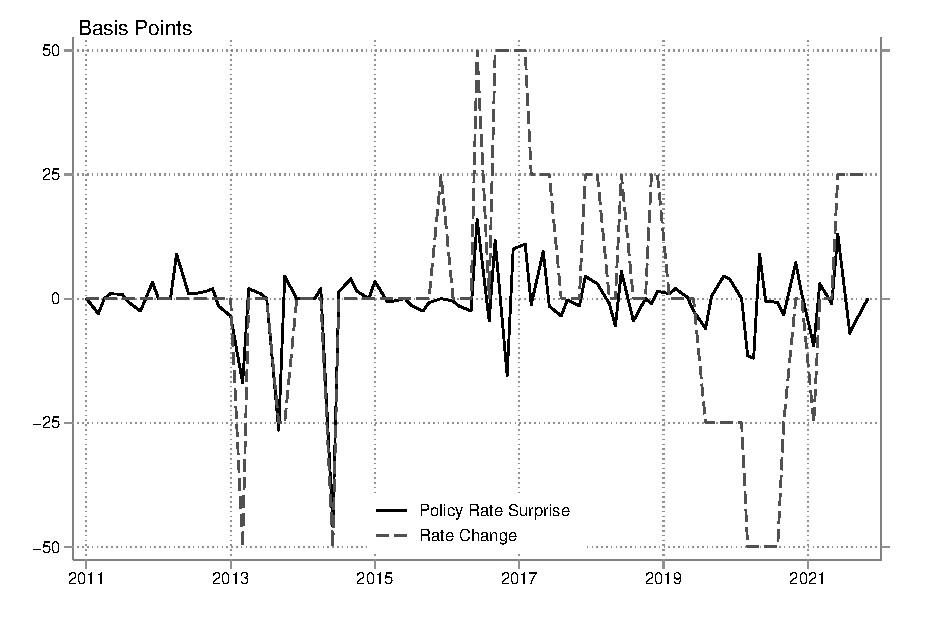
\includegraphics[width=1\textwidth,height=.3\textheight]{../Figures/prshocks.eps} \\
				\end{center}
				\fignotes{This figure compares the evolution of the surprises (solid line) and the raw changes (dashed line) in the policy rate. The surprises are the change in the 3-month swap in 30-minute windows bracketing monetary policy announcements from January 2011 to \lastobsfx.}
			\end{minipage}
		\end{center}
	\end{figure}
}

\clearpage
\afterpage{
	\begin{figure}[t]
		\caption{Persistence of the Exchange Rate Response to Policy Rate Surprises} \label{fig:persistprsfx}
		\begin{center}								% center the minipage on the line
			\begin{minipage}{0.9\linewidth}
				\begin{center}							% center the figure inside the minipage
					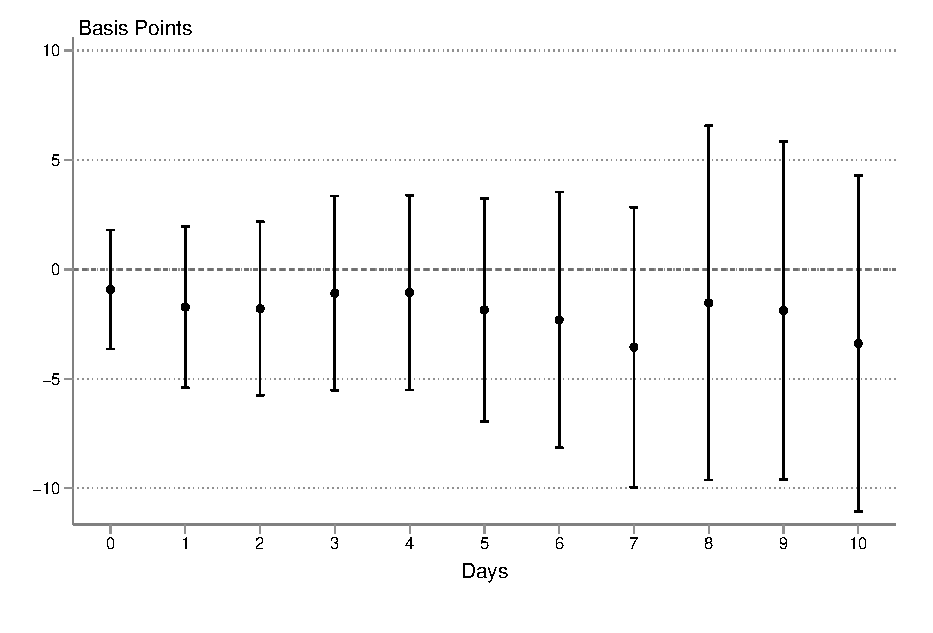
\includegraphics[trim={0.5cm 0cm 0.5cm 0cm},clip,height=.2\textheight,width=1\textwidth]{../Figures/persistprsusdmxn.eps} \\
				\end{center}
				\fignotes{This figure plots the coefficient estimates and 95\% confidence intervals for the response of the exchange rate returns to policy rate surprises. Returns are calculated from close of day \(t - 1\) to day \(t + \idxh\), where \(t\) is a day with a monetary policy announcement and \(\idxh = 0, 1, \ldots, 10\). Announcements are more than ten days apart from each other, see appendix \ref{sec:calendar}. The sample includes all regular monetary policy announcements from January 2011 to \lastobsfx.} 
			\end{minipage}
		\end{center}
	\end{figure}
}

\clearpage
\renewcommand\thefigure{\ref{sec:yieldcurve}\arabic{figure}}
\setcounter{figure}{0}
\begin{figure}[tbph]
	\caption{Persistence of the Yield Curve Response to Policy Rate Surprises} \label{fig:persistprsyc}
	\begin{center}								% center the minipage on the line
		\begin{minipage}{0.9\linewidth}
			\begin{center}							% center the figure inside the minipage
				\label{fig:persistprsyc}
				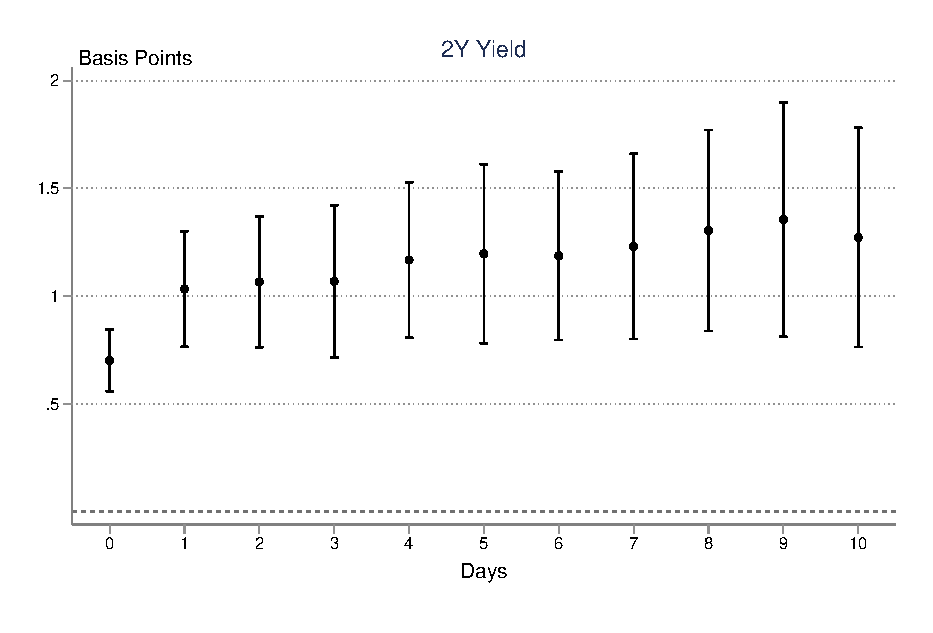
\includegraphics[trim={0.5cm 0cm 0.5cm 0cm},clip,height=.2\textheight,width=1\textwidth]{../Figures/persistprsgmxn02yr.eps} \\
				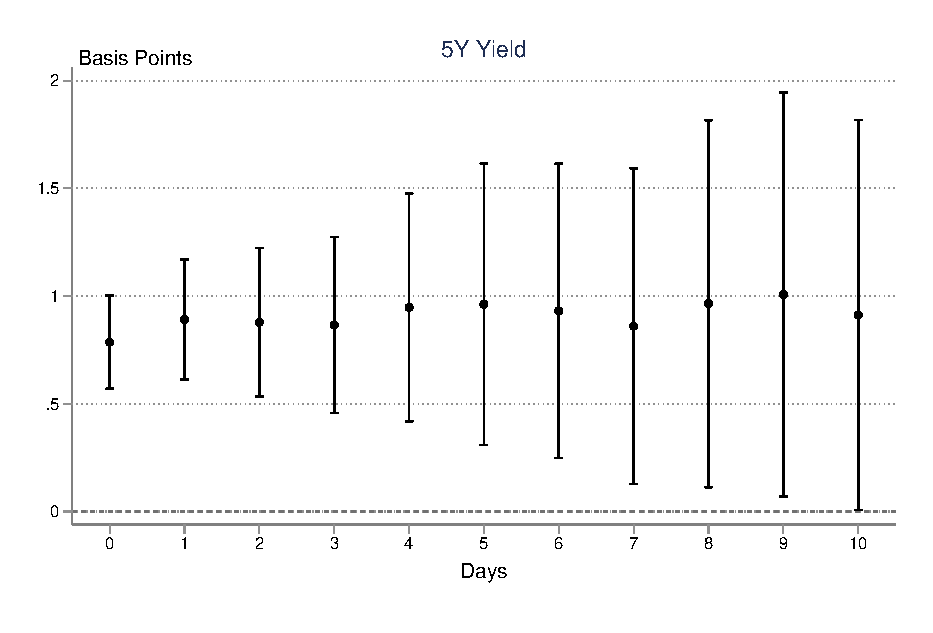
\includegraphics[trim={0.5cm 0cm 0.5cm 0cm},clip,height=.2\textheight,width=1\textwidth]{../Figures/persistprsgmxn05yr.eps} \\
				\includegraphics[trim={0.5cm 0cm 0.5cm 0cm},clip,height=.2\textheight,width=1\textwidth]{../Figures/persistprsgmxn10yr.eps} \\
				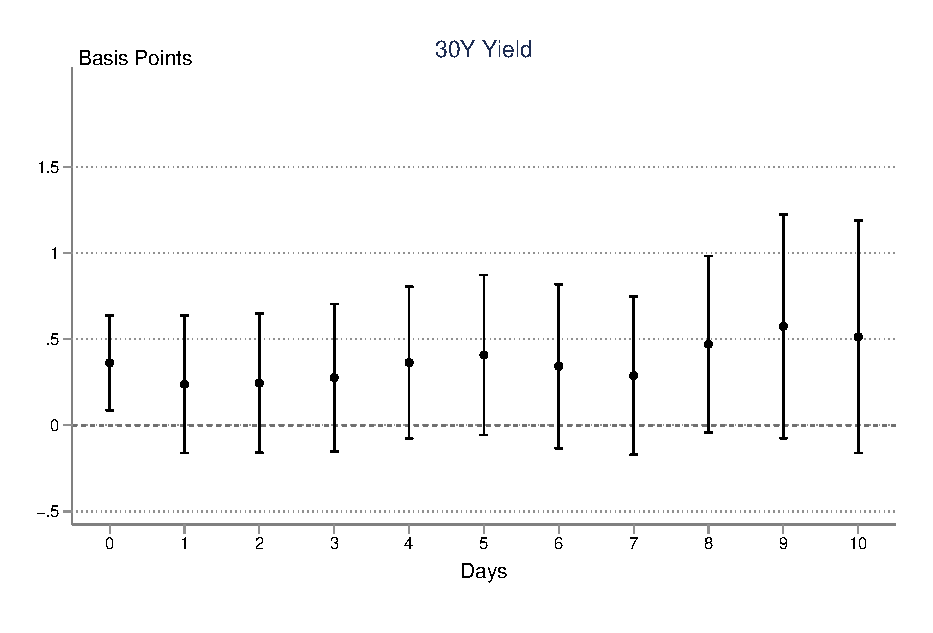
\includegraphics[trim={0.5cm 0cm 0.5cm 0cm},clip,height=.2\textheight,width=1\textwidth]{../Figures/persistprsgmxn30yr.eps} \\
			\end{center}
			\fignotes{This figure plots the coefficient estimates and 95\% confidence intervals for the response of the 2-, 5-, 10- and 30-year yields to policy rate surprises. Yield changes are calculated from close of day \(t - 1\) to day \(t + \idxh\), where \(t\) is a day with a monetary policy announcement and \(\idxh = 0, 1, \ldots, 10\). Announcements are more than ten days apart from each other, see appendix \ref{sec:calendar}. The sample includes all regular monetary policy announcements from January 2011 to \lastobsfx.}
		\end{minipage}
	\end{center}
\end{figure}

\end{document}

%---------------------------------------------------------------
% CRediT (Contributor Roles Taxonomy) author statement
%---------------------------------------------------------------
% Pavel Solís: Conceptualization, methodology, data curation, formal analysis, investigation, software, validation, visualization, writing.
% Jonathan Wright: Supervision.